\documentclass[12pt,fontset=fandol]{ctexart}
% 基础宏包与数学命令
% Basic packages and shared math macros

% 基础符号与文本环境
% Core symbols and text utilities
\usepackage{latexsym}
\usepackage{enumerate}
\usepackage{verbatim}

% 中文文档与页面版式
% Chinese document support and page layout
\usepackage{fontspec}
\usepackage{geometry}
\geometry{a4paper,left=2.5cm,right=2.5cm,top=2.5cm,bottom=2.5cm}

% 数学排版与公式环境
% Math typesetting and formula environments
\usepackage{amsmath}
\usepackage{amssymb}
\usepackage{amsfonts}
\usepackage{amsthm}
\usepackage{mathrsfs}
\usepackage{bm}
\usepackage[subnum]{cases}

% 图表与浮动体
% Figures, tables, and floating objects
\usepackage{float}
\usepackage{booktabs}
\usepackage{longtable}
\usepackage{multirow}
\usepackage{setspace}
\usepackage{graphicx}
\graphicspath{{figure/}}
\usepackage{subcaption}
\usepackage[dvipsnames]{xcolor}

% 算法、代码与填充文本
% Algorithms, code listings, and filler text
\usepackage{algorithm}
\usepackage{algorithmic}
\usepackage{lipsum}
\usepackage{listings}
\usepackage[framed,numbered,autolinebreaks,useliterate]{mcode}

% 其他常用工具
% Other common utilities
\usepackage{hyperref}
\hypersetup{hypertex=true,
colorlinks=true,
linkcolor = black,
anchorcolor = black,
citecolor = black}
\usepackage{cleveref}
\crefname{figure}{\textcolor{blue!80!black}{图}}{\textcolor{blue!80!black}{图}}
\crefname{table}{\textcolor{blue!80!black}{表}}{\textcolor{blue!80!black}{表}}
\crefname{equation}{\textcolor{blue!80!black}{式}}{\textcolor{blue!80!black}{式}}
\crefname{algorithm}{\textcolor{blue!80!black}{算法}}{\textcolor{blue!80!black}{算法}}

% 常用数学算子
% Common math operators
\DeclareMathOperator*{\argmin}{arg\,min}
\DeclareMathOperator*{\argmax}{arg\,max}
\DeclareMathOperator*{\minimax}{minimax}
\DeclareMathOperator{\diag}{diag}
\DeclareMathOperator{\tr}{tr}
\DeclareMathOperator{\rank}{rank}
\DeclareMathOperator{\Span}{Span}
\DeclareMathOperator{\range}{range}
\DeclareMathOperator{\nullspace}{null}
\DeclareMathOperator{\sign}{sign}
\DeclareMathOperator{\sgn}{sgn}
\DeclareMathOperator{\dist}{dist}
\DeclareMathOperator{\diam}{diam}

% 常用微分和向量记号
% Common differential and vector notation
\newcommand{\curl}{\text{\bf curl }}
\newcommand{\dx}{\mathrm{d}x}
\newcommand{\dy}{\mathrm{d}y}
\newcommand{\dz}{\mathrm{d}z}
\newcommand{\ds}{\mathrm{d}s}
\newcommand{\dS}{\mathrm{d}S}
\newcommand{\dt}{\mathrm{d}t}
\newcommand{\dd}{\d}
\renewcommand{\d}{\mathrm{d}}

% 定理环境
% Theorem environments
\newtheorem{definition}{\hspace{2em}定义}
\newtheorem{theorem}{\hspace{2em}定理}
\newtheorem{lemma}{\hspace{2em}引理}
\newtheorem{corollary}{\hspace{2em}推论}[section]
\renewcommand{\proofname}{\hspace{2em}证明}

% TikZ 绘图库
% TikZ libraries
\usepackage{tikz}
\usetikzlibrary{positioning}
\usetikzlibrary{arrows}
\usetikzlibrary{arrows.meta}
\usetikzlibrary{shapes.geometric,arrows}
\tikzset{ellbox/.style = {ellipse, draw=black, fill=blue!10}}

% 标题格式：一级标题四号黑体居中，二/三级标题小四号黑体左对齐
\ctexset{
    section = {
        format = \zihao{4}\heiti\centering,
    },
    subsection = {
        format = \zihao{-4}\heiti\raggedright,
    },
    subsubsection = {
        format = \zihao{-4}\heiti\raggedright,
    }
}

% 正文单倍行距
\singlespacing

% 页面格式设置
% Page formatting

% 页面编号：首页无页码，正文从第2页开始编页码（页脚居中）
\usepackage{fancyhdr}
\fancyhf{}
\fancyfoot[C]{\thepage}
\renewcommand{\headrulewidth}{0pt}
\pagestyle{fancy}

% 自定义标题页样式：
% 1. 三号黑体居中加粗
% 2. 不显示作者和日期
% 3. 标题页不显示页码
\makeatletter
\renewcommand*\maketitle{%
    \begin{center}%
        {\zihao{3}\heiti\bfseries \@title \par}
        \vskip 1em%
        {\global\let\author\@empty}%
        {\global\let\date\@empty}%
        \thispagestyle{empty}%
    \end{center}%
    \setcounter{footnote}{0}%
}
\makeatother

\def\q{\quad}




\title{医药冷链物流运输优化模型研究}



\begin{document}
	\maketitle

\vspace{1em}

\begin{center}
{\zihao{4}\heiti 摘\quad 要}
\end{center}

\vspace{0.5em}

本文围绕医药冷链物流运输优化问题，分别从运输成本核算、拼车路线优化和派车合理性评估三个层面展开研究。针对附件1的车辆成本参数和附件2的排货信息，建立了改进的运输成本核算模型；在此基础上，利用Clarke-Wright节约算法实现了拼车运输优化；针对附件3和附件4的大规模运单与派车数据，构建了基于熵权法的六维评估指标体系，并提出了三层递进优化方案。

{\bf 对于问题一：} 建立了区域差异化的往返运输成本核算模型。使用Haversine球面距离公式，结合东部（1.25）、中部（1.40）、西部（1.60）三区域的道路绕行系数估算实际道路距离。成本模型区分可变成本（油费、路桥费）与固定成本（人工、保险、审验、违章、胎耗、维保、折旧），考虑回程空载油耗系数0.75、工作天（280天）与日历天（365天）的差异化分摊以及车辆折旧。计算结果表明，2018年8月24日至11月23日期间，南通仓库共完成294趟运输，覆盖43个城市，运输总费用为3,846,906.89元。其中可变成本占48.1\%，固定成本占51.9\%；7.6M车型承担了93.2\%的运输趟次；东部地区成本占45.9\%，中部占26.2\%，西部占27.9\%。

{\bf 对于问题二：} 在问题一成本模型基础上，建立了带方向约束和距离约束的Clarke-Wright拼车优化模型。通过方位角方向聚类筛选可行合并对，计算节约值并施加容量约束（7.6M型11托、9.6M型14托）、方向偏离约束（≤90°）、城市间距离约束（≤500\,km）和组内跨度约束（≤120°），使用TSP排序优化各路线访问顺序。72组参数网格搜索的结果表明，最优参数组合下，运输路线从294条减至127条（减少56.8\%），总成本从3,846,906.89元降至1,706,894.88元，节约金额2,140,012.02元，节约率达55.63\%。

{\bf 对于问题三：} 建立了涵盖配送密度（分层市内/干线基准）、路线合并潜力、时效达标率、线路集中度、冷链合规率和装载饱和度六维指标的评估体系。采用熵权法根据各指标在54个仓库间的信息差异程度客观赋权，得到路线合并潜力权重最高（34.91\%）、时效达标率权重最低（1.37\%）的权重分配。系统加权综合得分为50.0分（满分为100分），评级为"需改进"。识别出23个仓库存在冷链合规率低于50\%的系统性风险。在优化方面，实施三层递进方案——TSP路径排序（节约5.6\%）、同城同日合并与车型优化匹配（冷链车辆强制约束），最终将周度总成本从1,135.3万元降至717.5万元，节约率达36.8\%。

{\bf 三个问题存在严密的逻辑递进关系：}问题一首先建立了改进的运输成本核算模型，为后续优化提供了精确的距离计算、成本构成分析以及数据预处理基础；问题二在问题一成本模型的基础上，利用Clarke-Wright节约算法并引入方向约束、距离约束等机制，实现了拼车运输的高效优化，进一步降低了运营成本；问题三则进一步拓展至终端配送场景，构建了基于熵权法的六维评估指标体系，并提出了三层递进优化方案，从而形成了从成本精确核算，到路线优化，再到派车方案评估与改进的完整逻辑链条。

\vspace{1em}

\newpage
\setcounter{page}{1}

\section{问题重述}\label{sec:problem-statement}
某大型医药流通企业在全国范围内运营着覆盖广泛的物流网络，包括5个枢纽仓库、41家省级仓库和200余家地市级仓库，自有车辆超过2000辆（其中冷藏车400余辆），终端配送覆盖100000余家药房和10000余家医院。在药品配送过程中，冷链药品对运输工具和时效有严格要求——除普通药品可使用常温车外，其余药品均需使用冷藏车运输，且送货时限通常允许3至4天，最长不超过一周。

本次竞赛围绕该企业的冷链药品运输优化展开，包含三个递进问题：

\textbf{问题一：运输费用分析。} 根据附件1提供的车辆运营成本与承载能力参数，以及附件2给出的南通市崇川区某医药企业仓库出发的冷链药品排货信息，建立运输成本核算模型，分析计算相应的运输总费用。

\textbf{问题二：拼车优化运输。} 在问题一的基础上，通过拼车（即多批货物合并运输）降低运营成本。装卸货工作时间限制为每日9:00至17:00，每次装卸约需2小时。假设所有订单信息可提前一周预知，设计改进的拼单运输和车辆调度方案，实现运输成本的最小化。

\textbf{问题三：派车单评估与优化。} 根据附件3提供的某一周终端运单需求数据和附件4给出的仓库至终端派车单数据，建立合理的评估指标体系，评价当前派车单安排的合理性，并在保证取送货时限的前提下提出优化方案。
˜

\section{问题分析}\label{sec:problem-analysis}
\subsection{问题一的分析}

问题一的核心任务是基于附件1和附件2的数据，精确计算冷链药品运输的总费用。该问题的关键在于：（1）从排货信息中准确提取目的地城市，并将其映射到地理坐标以计算运输距离；（2）建立符合实际运营逻辑的运输成本模型。基础的直线距离计算可采用Haversine球面距离公式，但实际道路距离需要考虑绕行因素，且不同地区（东部、中部、西部）的道路网络密度差异较大，应采用区域差异化的绕行系数。成本模型需要区分可变成本（油费、路桥费）和固定成本（人工、保险、折旧等），在往返运输场景下还要考虑回程空载带来的油耗下降。问题一属于数据驱动的成本核算问题，求解的关键在于数据清洗的鲁棒性和成本分摊逻辑的合理性。

\subsection{问题二的分析}

问题二要求在问题一的成本模型基础上，通过拼车合并运输实现成本节约。这是一个带容量约束的车辆路径问题（Capacitated Vehicle Routing Problem, CVRP）的变体：从单一仓库出发，需要将分布在不同城市的订单合并为尽可能少的运输路线。与标准CVRP的区别在于：（1）成本函数是非线性的——车辆选择（4.2M/7.6M/9.6M三种冷藏车）影响单位成本和载货容量，需匹配实际货物托盘数；（2）存在方向可行性约束——只有方向相近的目的地才适合拼车，否则绕行成本将抵消节约；（3）存在时间窗口约束——每日装卸时间仅8小时（9:00–17:00），每次装卸2小时。考虑到数据中存在自然的"周"分组结构，可逐周进行优化，并探索相邻周之间的跨周合并空间。Clarke-Wright节约算法因其计算效率高、易于施加方向约束的特性，适合本问题的求解。TSP路径排序（最近邻构造+2-opt改进）可用于优化同一路线内的访问顺序。

\subsection{问题三的分析}

问题三的性质与问题一、二不同——它不直接求解一个优化问题，而是先评估现有方案的合理性，再提出改进。数据规模更大（一周约53.6万条运单、22.2万条派车记录），涉及152个城市、88个仓库。评估的核心挑战在于：（1）设计合理的评估指标体系——不能主观判断，需要从配送效率、路线质量、时效表现、需求结构、合规水平等多个维度综合度量；（2）权重的确定——不同指标的重要程度不同，且应避免主观赋权带来的偏差。熵权法是一种基于数据本身差异程度的客观赋权方法：指标在各仓库间的差异越大，说明该指标的区分能力越强，应赋予更高权重。优化方面，派车单安排存在三层改进空间：单车辆日内的TSP路径排序→同一仓库同一天内不同车辆间的订单合并→合并后路线与最优车型的匹配。

\subsection{流程分析}

整体求解流程如下：首先进行数据预处理，包括城市名提取、地理坐标匹配、运输趟次/车辆日聚合；然后分别针对三个问题建立模型——问题一的改进运输成本核算模型、问题二的Clarke-Wright拼车优化模型、问题三的熵权法合理性评估模型与三层递进优化模型；接着求解并输出数值结果；最后进行模型评价。三问题之间存在递进关系：问题一提供基础成本核算框架，问题二在此基础上引入拼车优化，问题三则将评估与优化拓展到多仓库、多终端的大规模实际运作场景。


\section{模型中的假设与符号}\label{sec:assumptions-and-symbols}
\subsection{模型假设}

\begin{enumerate}
    \item \label{as:road} 实际道路距离与球面直线距离之间满足固定的区域比例关系。将全国城市按东部、中部、西部分别设定绕行系数 $\beta_E = 1.25$、$\beta_M = 1.40$、$\beta_W = 1.60$，同一区域内所有城市共享相同绕行系数。
    \item \label{as:speed} 车辆在高速公路上以平均速度 $v_h = 70\,\mathrm{km/h}$ 匀速行驶（问题一、二），在含城市道路的混合路况下以 $v_c = 60\,\mathrm{km/h}$ 匀速行驶（问题三），忽略交通拥堵、天气等随机因素。
    \item \label{as:load} 每次装卸货作业固定耗时 $t_{\mathrm{lu}} = 2\,\mathrm{h}$，装卸货工作仅能在每日9:00至17:00之间进行，单日最多可完成4次装卸操作。
    \item \label{as:empty} 车辆回程空载时油耗为满载油耗的75\%（空载系数 $\alpha = 0.75$），路桥费与去程相同，人工等固定成本不受负载影响。
    \item \label{as:week} 问题二中，所有订单信息可提前一周完整预知，允许在同一自然周内自由组合拼车，且相邻周之间可在满足时效约束的前提下进行跨周合并。
    \item \label{as:single} 问题二仅考虑从南通单一仓库出发的运输场景；问题三中，各仓库独立运作，仓库之间不存在库存调拨或跨仓库订单协同。
    \item \label{as:capacity} 每辆冷藏车的承载能力以托盘数为单位：4.2M型5托，7.6M型11托，9.6M型14托。一条拼车路线内各城市货物托盘数之和不超过所选车型的容量上限。
    \item \label{as:cold} 冷链药品（非"普通药品"类）必须由冷藏车运输；普通药品既可使用常温车，也可使用冷藏车。违反冷链规定的配送被视为不合规。
    \item \label{as:driver} 驾驶员每日驾驶时间不超过10小时，连续行驶允许中途休息，但路线总运输天数由累计驾驶时间和装卸次数共同决定。
    \item \label{as:depot} 所有运输趟次从仓库出发，按规划路线访问各目的地后返回原仓库（闭合路线），不考虑中途补货或临时更改路线。
\end{enumerate}


\subsection{符号约定}

模型中所用符号的含义以及单位见\cref{tab:signal}。
\begin{table}[h]
    \caption{符号约定}\label{tab:signal} \centering
    \begin{tabular}{ccc}
        \toprule[1.5pt]
        符号 & 含义 & 单位 \\
        \midrule[1pt]
        $(\varphi, \lambda)$ & 仓库或城市的经纬度坐标 & $({}^\circ,{}^\circ)$ \\
        $d_{\mathrm{s}}(A,B)$ & 城市 $A$ 与 $B$ 之间的球面直线距离 & km \\
        $R$ & 地球平均半径 ($R = 6371$) & km \\
        $\beta_r$ & 区域 $r$ 的道路绕行系数 & — \\
        $d_{\mathrm{r}}(A,B)$ & 城市 $A$ 与 $B$ 之间的道路估算距离 & km \\
        $\theta_i$ & 从出发仓库看向城市 $i$ 的方位角 & ${}^\circ$ \\
        $\alpha$ & 回程空载油耗系数 ($\alpha = 0.75$) & — \\
        $C_{\mathrm{var}}$ & 单位距离可变成本（油费 + 路桥费）& 元/km \\
        $C_{\mathrm{fix}}$ & 每日固定成本（人工 + 保险 + 审验 + 违章 + 胎耗 + 维保 + 折旧）& 元/天 \\
        $n_v$ & 运输所需车辆数 & 辆 \\
        $T_{ij}$ & 城市 $i$ 到城市 $j$ 的运输天数 & 天 \\
        $p_i$ & 城市 $i$ 的货物托盘数 & 托 \\
        $Q_v$ & 车型 $v$ 的最大承载托数 & 托 \\
        $s_{ij}$ & 合并城市 $i$ 与 $j$ 的CW节约值 & 元 \\
        $\theta_d$ & 方向偏离角阈值 & ${}^\circ$ \\
        $d_{\max}$ & 城市间距离合并上限 & km \\
        $\theta_g$ & 合并组内城市的方位角跨度上限 & ${}^\circ$ \\
        $m_k$ & 路线 $k$ 中访问的城市数 & 个 \\
        $D_k$ & 路线 $k$ 的往返总道路距离 & km \\
        $T_k$ & 路线 $k$ 的运输天数 & 天 \\
        $S_{kj}$ & 仓库 $k$ 在指标 $j$ 上的绝对得分 & 分 \\
        $w_j$ & 指标 $j$ 的熵权权重 & — \\
        $e_j$ & 指标 $j$ 的信息熵 & — \\
        $F_k$ & 仓库 $k$ 的综合得分 & 分 \\
        $F_{\mathrm{sys}}$ & 系统加权综合得分 & 分 \\
        \bottomrule[1.5pt]
    \end{tabular}
\end{table}


\section{模型的建立}\label{sec:model-construction}
\subsection{运输成本核算模型}

\subsubsection{球面距离与道路距离}

从仓库出发至目的地的运输距离是成本计算的基础。设出发点（南通市崇川区）经纬度为 $(\varphi_0, \lambda_0) = (31.98^\circ\mathrm{N}, 120.90^\circ\mathrm{E})$，目的地城市 $i$ 的经纬度为 $(\varphi_i, \lambda_i)$，使用Haversine公式\cite{sinnott1984haversine}计算两点间的球面大圆距离：

\begin{equation}\label{eq:haversine}
d_{\mathrm{s}} = 2R \arcsin\!\left(\sqrt{\sin^2\!\left(\frac{\Delta\varphi}{2}\right) + \cos\varphi_0 \cos\varphi_i \sin^2\!\left(\frac{\Delta\lambda}{2}\right)}\right)
\end{equation}

其中 $R = 6371\,\mathrm{km}$ 为地球平均半径，$\Delta\varphi = \varphi_i - \varphi_0$，$\Delta\lambda = \lambda_i - \lambda_0$。

实际道路距离通常大于球面直线距离，且不同地形区域的道路网络密度差异明显。为此引入区域差异化的道路绕行系数 $\beta_r$\cite{ballou2002circuity}：

\begin{equation}\label{eq:road}
d_{\mathrm{r}} = \beta_r \cdot d_{\mathrm{s}},\qquad \beta_r = \begin{cases}
1.25, & \text{东部地区}\\
1.40, & \text{中部地区}\\
1.60, & \text{西部地区}
\end{cases}
\end{equation}

\subsubsection{运输成本构成}

每趟运输的总成本由可变成本和固定成本两大部分构成。对于往返运输，去程满载、回程空载：

\textbf{可变成本（往返）：} 包括油费和路桥费。去程按满载计，回程空载油耗降为满载的 $\alpha$ 倍（$\alpha = 0.75$）\cite{coyle2006transportation}，路桥费不受负载影响：

\begin{equation}\label{eq:var}
\begin{aligned}
C_{\mathrm{var}}^{\mathrm{round}} &= C_{\mathrm{var}}^{\mathrm{out}} + C_{\mathrm{var}}^{\mathrm{return}}\\
&= C_{\mathrm{var}}^{\mathrm{per\_km}} \cdot d_{\mathrm{r}} + \left(\alpha \cdot C_{\mathrm{fuel}}^{\mathrm{per\_km}} + C_{\mathrm{toll}}^{\mathrm{per\_km}}\right) \cdot d_{\mathrm{r}}
\end{aligned}
\end{equation}

\textbf{固定成本（往返）：} 人工成本、保险、审验、违章、轮胎损耗、维修保养和折旧七项在往返两程各计一次（共2倍），其中各项按不同的摊销周期转换为日成本：

\begin{equation}\label{eq:fix_items}
\begin{aligned}
C_{\mathrm{labor}}^{\mathrm{day}} &= \frac{\text{人工年成本}}{280} \quad (\text{工作天})\\
C_{\mathrm{ins}}^{\mathrm{day}} &= \frac{\text{保险年成本}}{365} \quad (\text{日历天})\\
C_{\mathrm{insp}}^{\mathrm{day}} &= \frac{\text{审验年成本}}{365} \quad (\text{日历天})\\
C_{\mathrm{viol}}^{\mathrm{day}} &= \frac{\text{违章年成本}}{365} \quad (\text{日历天})\\
C_{\mathrm{tire}}^{\mathrm{day}} &= \frac{\text{轮胎年成本}}{280} \quad (\text{工作天})\\
C_{\mathrm{maint}}^{\mathrm{day}} &= \frac{\text{维保年成本}}{300} \quad (\text{维保天})\\
C_{\mathrm{depr}}^{\mathrm{day}} &= \frac{\text{车辆购置价} - \text{报废补贴}}{4 \times 280} \quad (\text{4年折旧, 工作天})
\end{aligned}
\end{equation}

每日固定成本总和为 $C_{\mathrm{fix}}^{\mathrm{day}} = \sum C_{\mathrm{*}}^{\mathrm{day}}$。往返固定成本为：

\begin{equation}\label{eq:fix}
C_{\mathrm{fix}}^{\mathrm{round}} = 2 \cdot C_{\mathrm{fix}}^{\mathrm{day}} \cdot T
\end{equation}

其中 $T$ 为往返运输天数，由单程距离和驾驶速度估算。

\textbf{单趟运输总成本：} 综合以上各部分，一趟运输的总成本为：

\begin{equation}\label{eq:trip_cost}
C_{\mathrm{trip}} = C_{\mathrm{var}}^{\mathrm{round}} + C_{\mathrm{fix}}^{\mathrm{round}}
\end{equation}

\textbf{运输总费用：} 所有运输趟次的成本之和：

\begin{equation}\label{eq:total_cost}
C_{\mathrm{total}} = \sum_{k=1}^{N} C_{\mathrm{trip}}^{(k)}
\end{equation}

\subsection{Clarke-Wright拼车优化模型}

\subsubsection{方向聚类与可行性约束}

拼车的前提是多个目的地城市在同一条合理的路径上。首先计算各城市相对于出发点的方位角\cite{bowditch2002navigator}：

\begin{equation}\label{eq:bearing}
\theta = \arctan\!2\Big(\sin(\Delta\lambda)\cos\varphi_i,\; \cos\varphi_0\sin\varphi_i - \sin\varphi_0\cos\varphi_i\cos(\Delta\lambda)\Big)
\end{equation}

对于任意两个城市 $i$ 和 $j$，拼车的可行性需满足以下约束：

\begin{enumerate}
    \item \textbf{方向可行性：}两城市的方位角差异不超过阈值 $\theta_d$，$|\theta_i - \theta_j| \leq \theta_d$。
    \item \textbf{距离可行性：}两城市之间的道路距离不超过上限 $d_{\max}$，$d_{\mathrm{r}}(i,j) \leq d_{\max}$。
    \item \textbf{组内跨度约束：}合并后的路线中，最大方位角与最小方位角之差不超过 $\theta_g$。
    \item \textbf{容量约束：}合并后路线中所有城市的货物托盘总数不超过所选车型的承载上限 $Q_v$。
\end{enumerate}

\subsubsection{CW节约算法}

对于符合可行性约束的两城市 $i$ 和 $j$，若将它们从分别独立往返合并为一条路线（从仓库依次访问 $i$ 和 $j$ 后返回），可节约的运输距离为：

\begin{equation}\label{eq:cw_saving_dist}
\Delta d_{ij} = d_{0i} + d_{j0} - d_{ij}
\end{equation}

节约的成本为距离节约带来的可变成本减少加上运输天数缩短带来的固定成本减少：

\begin{equation}\label{eq:cw_saving}
s_{ij} = C_{\mathrm{var}}^{\mathrm{per\_km}} \cdot \Delta d_{ij} + C_{\mathrm{fix}}^{\mathrm{day}} \cdot \Delta T_{ij}
\end{equation}

其中 $\Delta T_{ij}$ 为合并前后运输天数的变化。$s_{ij} > 0$ 时说明合并是有利可图的。

\subsubsection{算法流程}

CW算法以贪心方式构造路线合并：首先将所有城市视为独立的单点路线；计算所有可行城市对的节约值并按降序排序；依次处理每条候选边，若合并两端城市所属路线不违反可行性约束，则执行合并，将两条路线连接为一条更大的路线。合并过程中使用并查集维护路线归属。

\subsubsection{TSP路线排序}

对于每条包含 $m$ 个城市的合并路线，需确定从仓库出发访问所有城市并返回的最优顺序。采用最近邻构造算法生成初始路径，然后使用2-opt局部搜索进行改进：

\begin{enumerate}
    \item 从仓库出发，每次选择距当前城市最近、尚未访问的城市作为下一站；
    \item 重复直至所有城市访问完毕，返回仓库；
    \item 对所有可能的边对 $(p,q)$ 和 $(r,s)$ 执行2-opt交换（将边 $pq$ 和 $rs$ 替换为 $pr$ 和 $qs$），若交换后路径总距离缩短则保留，直至无法进一步改进。
\end{enumerate}

\subsubsection{多站路线成本计算}

完成路线排序后，路线 $k$ 的总往返距离 $D_k$ 为依次访问所有城市并返回仓库的道路距离之和。运输天数由驾驶时间和装卸时间共同决定：

\begin{equation}\label{eq:travel_days}
T_k = \max\!\left(1,\; \left\lceil \frac{D_k}{v_h \cdot H_d} + \frac{m_k \cdot t_{\mathrm{lu}}}{H_w} \right\rceil \right)
\end{equation}

其中 $v_h$ 为车辆平均行驶速度（单位：$\mathrm{km/h}$），$t_{\mathrm{lu}}$ 为单次装卸货时间（单位：$\mathrm{h}$），$H_d = 10\,\mathrm{h}$ 为每日驾驶时间上限，$H_w = 8\,\mathrm{h}$ 为每日装卸工作窗口。路线总成本按 \cref{eq:trip_cost} 计算，根据实际托盘数选择满足容量约束且成本最低的车型。

\subsection{熵权法派车合理性评估模型}

\subsubsection{六维评估指标体系}

从配送效率、路线质量、时效表现、需求结构、合规水平和运力利用六个维度构建评估指标体系：

\textbf{指标1——配送密度（分层，中间型指标）：} 区分市内配送和干线运输，分别以行业经验确定最优停靠点区间——市内配送并非停靠点越多越好，过多意味着单点服务时间不足、存在质量风险。市内以 $[12, 18]$ 点/日为最优区间，干线以 $[3, 5]$ 点/日为最优区间；区间内得满分，偏离两侧则线性扣分。各车辆的配送密度按类型分层后得分。

\textbf{指标2——路线合并潜力：} 对各仓库的配送目的地，计算使用CW算法可节约距离的比例，并将其线性映射到得分区间。

\textbf{指标3——时效达标率：} 根据运单中的运输时效要求（送货、次日送达、急送等），统计在时限内完成的订单占比。

\textbf{指标4——线路集中度：} 基于信息熵衡量各仓库运单在"线路号"维度上的分布集中程度。集中度高意味着订单集中在少数成熟线路上，易形成规模效应与标准化管理；集中度低意味着需求碎片化、线路分散，难以通过合并实现降本增效。

\textbf{指标5——冷链合规率：} 冷链药品订单中实际使用冷藏车配送的比例。冷链药品必须由冷藏车运输，常温车配送冷链订单视为不合规。

\textbf{指标6——车辆装载饱和度：} 以各车型（小型车、中型车、大型车、冷藏车）在全量数据中的第75百分位数装载量为基准，计算每个车辆日的装载量相对于该基准的饱和度。饱和度越高说明运力利用越充分，长期低于行业p75水平的仓库存在运力浪费。

各指标的得分通过行业基准映射函数转换为0至100分的绝对评分。以下给出各指标评分函数的具体计算公式。

{\bf 指标1——配送密度（分层，中间型指标）：}设仓库 $k$ 有 $n_k^c$ 个市内型车辆日和 $n_k^l$ 个干线型车辆日，两者的划分标准为：若某车辆日之市内停靠点数 $\geq$ 干线停靠点数，则归入市内型，否则归入干线型。记市内型车辆日的平均停靠点数为 $\bar{a}_k^c$，干线型车辆日的平均停靠点数为 $\bar{a}_k^l$。配送密度属于中间型指标——停靠点过少说明调度效率低、车辆空转严重；停靠点过多则意味着单点卸货时间被压缩、服务质量存疑。因此采用梯形隶属函数：最优区间内获满分，偏离两侧则线性递减。市内配送的最优区间为 $[12, 18]$ 点/日，干线运输的最优区间为 $[3, 5]$ 点/日：


\begin{equation}\label{eq:score_s1_city}
S_{k1}^c = \begin{cases}
\dfrac{\bar{a}_k^c}{12} \times 100, & \bar{a}_k^c < 12\\
100, & 12 \leq \bar{a}_k^c \leq 18\\
\max\!\left(100 - \dfrac{\bar{a}_k^c - 18}{18} \times 100,\; 0\right), & \bar{a}_k^c > 18
\end{cases}
\end{equation}

\begin{equation}\label{eq:score_s1_line}
S_{k1}^l = \begin{cases}
\dfrac{\bar{a}_k^l}{3} \times 100, & \bar{a}_k^l < 3\\
100, & 3 \leq \bar{a}_k^l \leq 5\\
\max\!\left(100 - \dfrac{\bar{a}_k^l - 5}{5} \times 100,\; 0\right), & \bar{a}_k^l > 5
\end{cases}
\end{equation}

{\bf 指标2——路线合并潜力：}对于仓库 $k$ 的每一个车辆日 $v$，设其目的地集合为 $D_v$（$|D_v| \geq 2$）。分别计算独立往返总距离 $\sum_{d \in D_v} 2 d_{\mathrm{r}}(0,d)$ 与TSP优化后路线总距离 $d_{\mathrm{tsp}}(D_v)$，该车辆日的距离节约比例为 $p_v = \dfrac{\sum_{d \in D_v} 2 d_{\mathrm{r}}(0,d) - d_{\mathrm{tsp}}(D_v)}{\sum_{d \in D_v} 2 d_{\mathrm{r}}(0,d)} \times 100\%$。取所有车辆日节约比例的均值 $\bar{p}_k$，并作线性映射至得分区间：

\begin{equation}\label{eq:score_s2}
S_{k2} = \min\!\bigl(\max\!\bigl(50 + \bar{p}_k,\; 0\bigr),\; 100\bigr)
\end{equation}

该设计使得节约率为50\%时获得满分100分，节约率为0\%时获得50分（及格线），节约率为负时降至50分以下。

{\bf 指标3——时效达标率：}设仓库 $k$ 的运单中共涉及 $M_k$ 个有时效要求的订单，其中在第 $m$ 个订单的规定时限内完成配送的订单数为 $M_k^{\text{ok}}$，则：

\begin{equation}\label{eq:score_s3}
S_{k3} = \frac{M_k^{\text{ok}}}{M_k} \times 100
\end{equation}

若无时效订单（$M_k = 0$），则记 $S_{k3} = 100$。

{\bf 指标4——线路集中度：}设仓库 $k$ 的运单共涉及 $L_k$ 条线路，第 $i$ 条线路的订单占比为 $p_i$（$\sum_{i=1}^{L_k} p_i = 1$）。定义线路分布的香农熵 $H_k = -\sum_{i=1}^{L_k} p_i \ln p_i$，其最大可能值为等分布时的 $\ln L_k$。则标准化集中度为：

\begin{equation}\label{eq:score_s4}
S_{k4} = \left(1 - \frac{H_k}{\ln L_k}\right) \times 100
\end{equation}

若 $L_k = 1$（所有订单集中在唯一线路上），则 $H_k = 0$，$S_{k4} = 100$；若所有线路均匀分布，则 $H_k = \ln L_k$，$S_{k4} = 0$。该指标衡量的是需求结构的成熟度——线路越集中，说明仓库拥有稳定的骨干线路网络，有利于批量运输与路线固化带来的效率提升。

{\bf 指标5——冷链合规率：}设仓库 $k$ 的运单中包含 $C_k$ 个冷链药品订单，其中实际使用了冷藏车配送的订单数为 $C_k^{\text{cold}}$，则：

\begin{equation}\label{eq:score_s5}
S_{k5} = \frac{C_k^{\text{cold}}}{C_k} \times 100
\end{equation}

若无冷链订单（$C_k = 0$），则记 $S_{k5} = 100$。冷链药品必须由冷藏车运输；常温车配送冷链订单即构成不合规。

{\bf 指标6——车辆装载饱和度：}对于仓库 $k$ 的每一个车辆日 $v$，设其车辆分类为 $c$（小型车、中型车、大型车或冷藏车），该车辆日的总装载件数为 $q_v$。以全体数据中各车型装载量的第75百分位数 $Q_{75}^c$ 为基准，定义该车辆日的装载饱和度为：

\begin{equation}\label{eq:load_sat}
s_v = \min\!\left(\frac{q_v}{Q_{75}^c} \times 100,\; 100\right)
\end{equation}

饱和度达到或超过100\%表示该车辆日的装载量已处于行业前25\%水平，运力利用充分。仓库 $k$ 的装载饱和度得分取全部车辆日饱和度的平均值：

\begin{equation}\label{eq:score_s6}
S_{k6} = \frac{1}{V_k} \sum_{v=1}^{V_k} s_v
\end{equation}

其中 $V_k$ 为仓库 $k$ 的车辆日总数。该指标衡量的是车辆运力利用效率——装载过少意味着运力浪费、单位运输成本偏高；接近或超过行业p75基准则表明运力利用充分。

\subsubsection{熵权法客观赋权}

熵权法基于各指标在仓库间得分的差异程度确定权重。差异越大的指标，提供的信息量越大，应赋予更高的权重\cite{shannon1948mathematical,郭显光1998熵权}。计算步骤如下：

\textbf{步骤一——数据归一化：} 将各仓库得分矩阵 $S = (S_{kj})_{n \times m}$（$n$ 个仓库，$m$ 个指标）进行极差归一化：

\begin{equation}\label{eq:normalize}
r_{kj} = \frac{S_{kj} - \min_k(S_{kj})}{\max_k(S_{kj}) - \min_k(S_{kj})}
\end{equation}

\textbf{步骤二——计算比重矩阵：}

\begin{equation}\label{eq:proportion}
p_{kj} = \frac{r_{kj}}{\sum_{k=1}^{n} r_{kj}}
\end{equation}

\textbf{步骤三——计算各指标的信息熵：}

\begin{equation}\label{eq:entropy}
e_j = -\frac{1}{\ln n} \sum_{k=1}^{n} p_{kj} \ln(p_{kj})
\end{equation}

当 $p_{kj} = 0$ 时，取 $p_{kj}\ln(p_{kj}) = 0$。

\textbf{步骤四——计算差异系数与权重：} 差异系数 $d_j = 1 - e_j$，指标权重为差异系数的归一化：

\begin{equation}\label{eq:weight}
w_j = \frac{d_j}{\sum_{j=1}^{m} d_j}
\end{equation}

\subsubsection{综合得分与系统评价}

各仓库的综合得分为各指标绝对得分的加权和：

\begin{equation}\label{eq:composite}
F_k = \sum_{j=1}^{m} w_j \cdot S_{kj}
\end{equation}

系统层面的总得分以各仓库的车辆日数为权重进行加权平均：

\begin{equation}\label{eq:system}
F_{\mathrm{sys}} = \frac{\sum_{k=1}^{n} N_k \cdot F_k}{\sum_{k=1}^{n} N_k}
\end{equation}

其中 $N_k$ 为仓库 $k$ 的车辆日数。此外，使用TOPSIS方法\cite{hwang1981multiple}计算各仓库与理想解和负理想解的贴近度，对综合得分排名进行辅助验证。

\subsubsection{三层递进优化模型}

针对派车安排的优化采用三层递进策略：

\textbf{第1层——TSP路径排序：} 对每个车辆日内访问的多个目的地，使用最近邻构造加2-opt改进算法重排访问顺序\cite{lin1965computer}，缩短单个车辆日的行驶总距离。

\textbf{第2层——同城同日合并：} 同一仓库在同一天可能有多个车辆独立配送相同方向的城市。将同一仓库、同一日期的常温车和冷链车分别合并，使用CW算法\cite{clarke1964scheduling}将多条车辆日合并为更少的路线，分离冷链与常温品类以符合冷链合规要求。

\textbf{第3层——车型最优匹配：} 合并后的路线货物总量可能发生变化，需要重新选择最优车型。对于冷链药品路线，强制选择冷藏车型；对于常温药品路线，在满足容量约束的前提下选择综合成本最低的车型。


\section{模型应用与问题求解}\label{sec:problem-solving}
\subsection{问题一的求解}

\subsubsection{数据预处理}

首先从附件1读取车辆成本参数（\cref{tab:vehicle-costs}），从附件2读取排货信息。附件2包含2018年8月24日至11月23日期间从南通仓库出发的732条排货记录，按运输单号聚合为294个运输趟次。通过8层地址解析策略（特殊地址映射、正则匹配"XX市"、子串匹配城市坐标库等），从原始排货地址中提取标准城市名，共覆盖43个城市。将城市名匹配至包含155个中国城市经纬度的坐标库，计算各趟次从南通出发的单程道路距离。

\begin{table}[!h]
    \centering
    \begin{tabular}{lccc}
        \toprule[1.5pt]
        成本项目 & 4.2M & 7.6M & 9.6M \\
        \midrule[1pt]
        购置价（元）& 193{,}453 & 263{,}991 & 339{,}359 \\
        报废补贴（元）& 12{,}000 & 12{,}000 & 12{,}000 \\
        油耗（L/100km）& 13 & 17 & 20 \\
        油费（元/km）& 1.00 & 1.40 & 1.70 \\
        路桥费（元/km）& 0.70 & 1.00 & 1.30 \\
        人工（元/年）& 168{,}000 & 168{,}000 & 168{,}000 \\
        保险（元/年）& 11{,}504 & 16{,}048 & 16{,}286 \\
        审验（元/年）& 1{,}650 & 1{,}749 & 1{,}749 \\
        违章（元/年）& 60{,}833 & 60{,}833 & 60{,}833 \\
        轮胎（元/年）& 1{,}800 & 3{,}000 & 3{,}000 \\
        维保（元/年）& 84{,}000 & 96{,}000 & 96{,}000 \\
        冷藏车容量（托）& 5 & 11 & 14 \\
        \bottomrule[1.5pt]
    \end{tabular}\caption{各型号车辆成本参数（附件1）}
    \label{tab:vehicle-costs}

\end{table}

\subsubsection{费用计算结果}

基于该成本模型计算，运输总费用为\textbf{3,846,906.89元}。其中可变成本（油费+路桥费，往返）1,848,938.21元（占48.1\%），固定成本（人工+摊销+折旧，往返）1,997,968.69元（占51.9\%）。固定成本与可变成本占比接近，说明两者在运输总成本中同等重要，如\cref{fig:cost_pie}：
\begin{figure}[!h]
    \centering
    % 第一张图
    \begin{subfigure}[b]{0.26\textwidth}
        \centering
        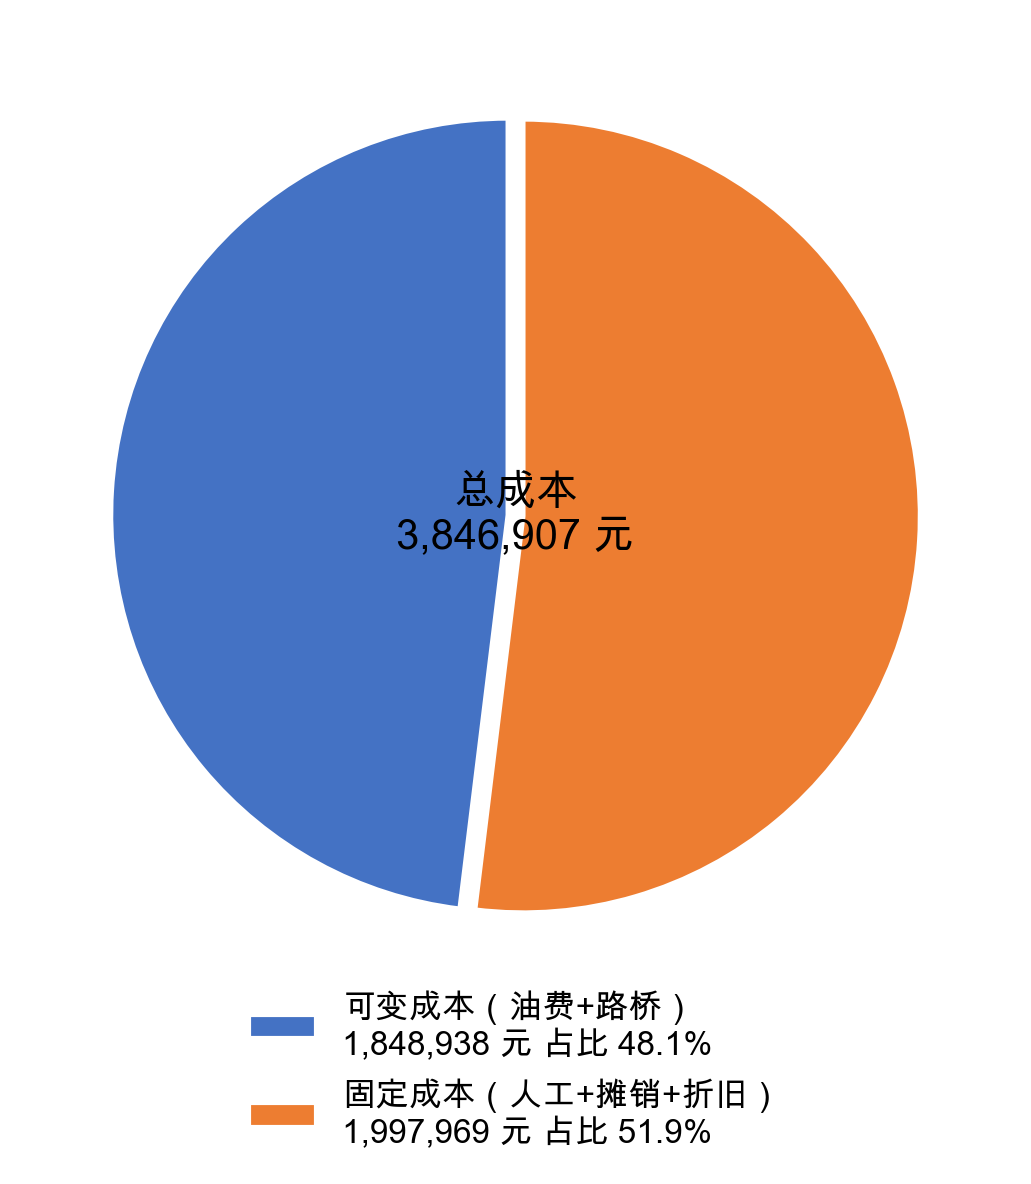
\includegraphics[width=\textwidth]{图1_问题一_成本构成饼图.png}
        \caption{运输成本总体构成}
        \label{fig:cost_pie}
    \end{subfigure}
    \hfill % 在子图之间插入弹性间距，使它们均匀分布
    % 第二张图
    \begin{subfigure}[b]{0.36\textwidth}
        \centering
        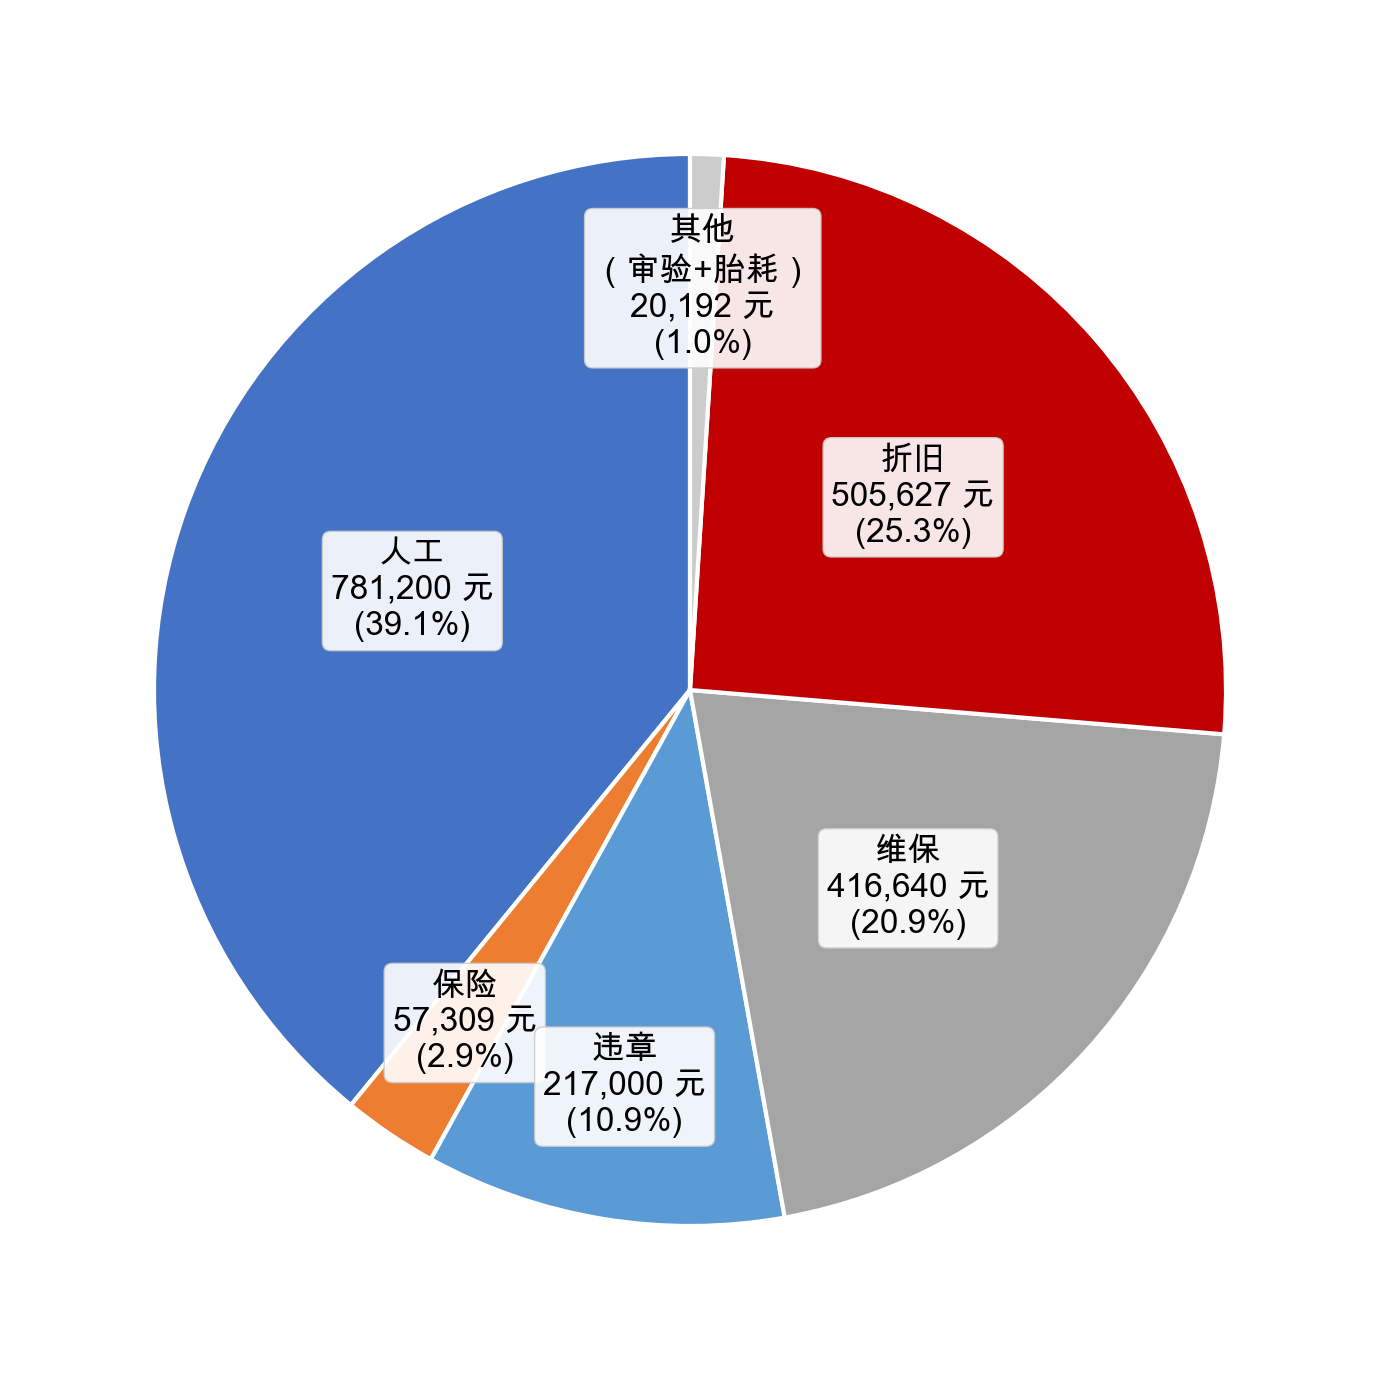
\includegraphics[width=\textwidth]{图7_固定成本构成饼图.png}
        \caption{固定成本构成}
        \label{fig:fixed_cost}
    \end{subfigure}
    \hfill
    % 第三张图
    \begin{subfigure}[b]{0.36\textwidth}
        \centering
        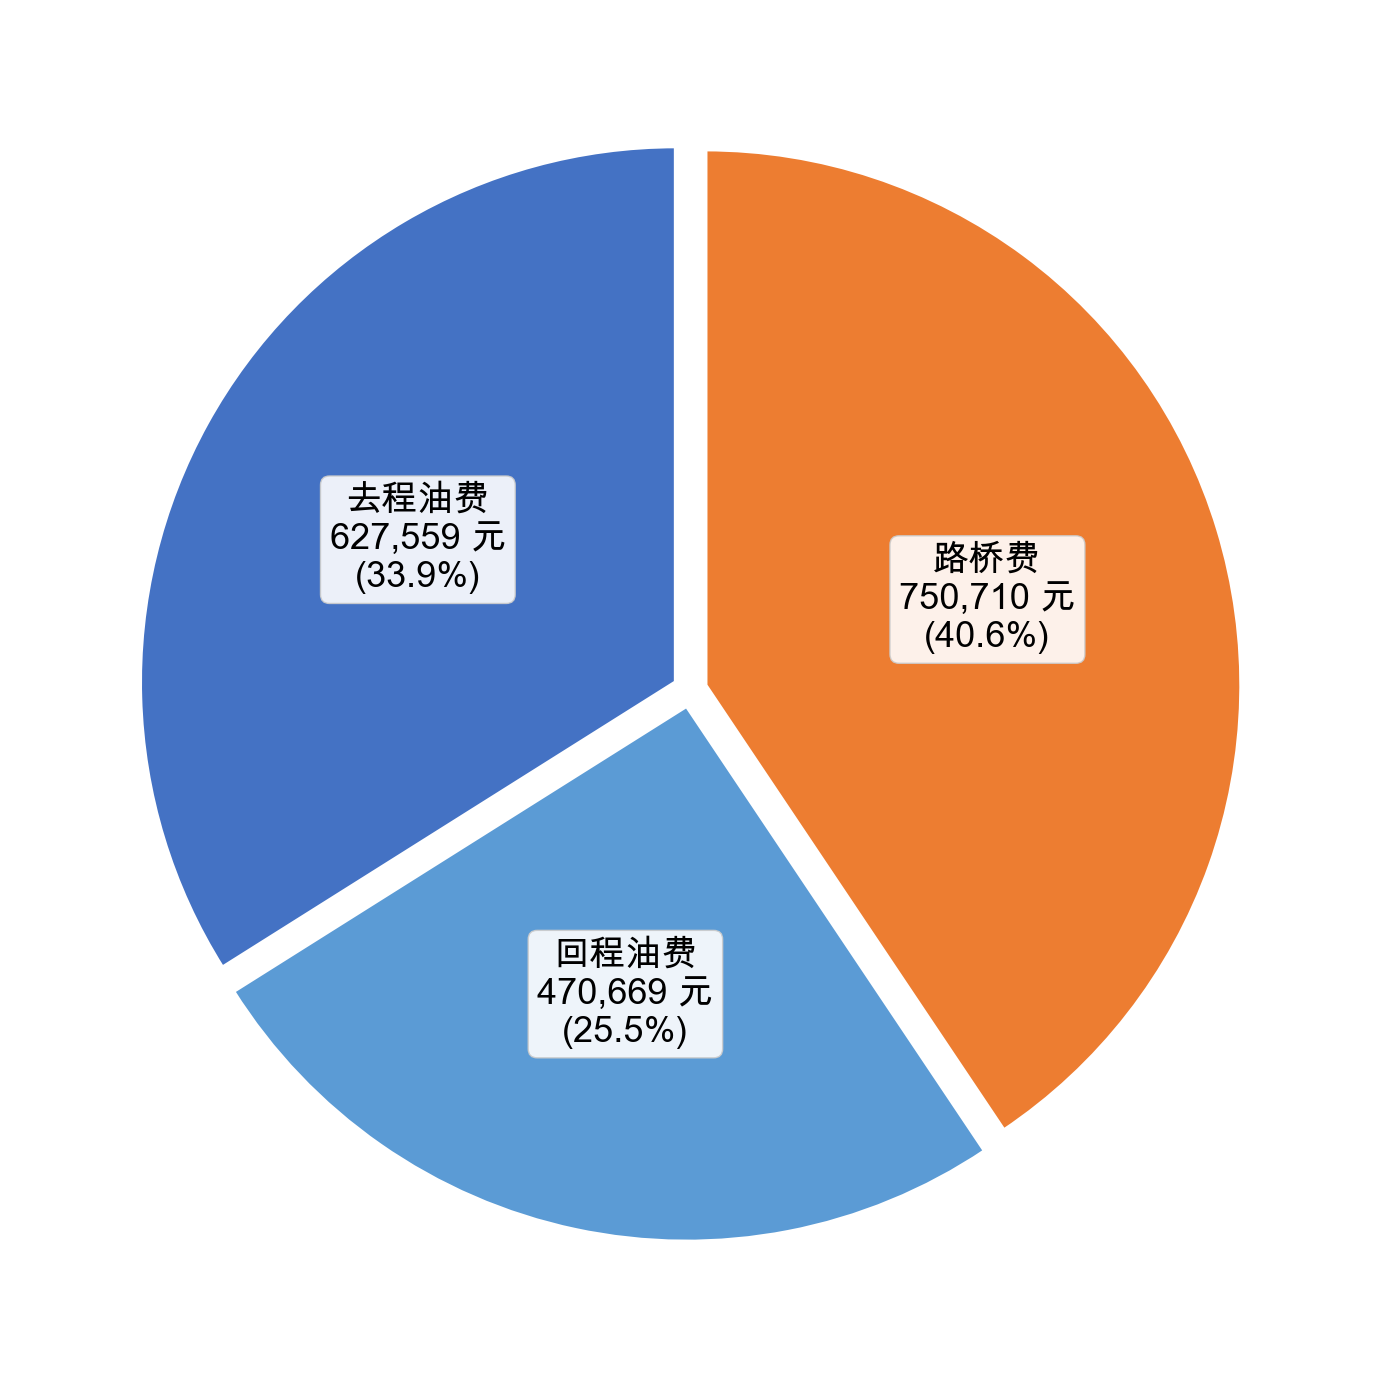
\includegraphics[width=\textwidth]{图8_可变成本构成饼图.png}
        \caption{可变成本构成}
        \label{fig:variable_cost}
    \end{subfigure}
    
    \caption{运输成本构成}
    \label{fig:total_figure}
\end{figure}

按车型统计（\cref{tab:by-vehicle}），7.6M冷藏车承担了274趟运输（93.2\%），9.6M承担了20趟（6.8\%），4.2M因容量较小未被选用。

\begin{table}[!h]
    \centering
    \begin{tabular}{lcccc}
        \toprule[1.5pt]
        车型 & 趟次数 & 占比 & 总成本（元）& 平均成本（元/趟）\\
        \midrule[1pt]
        7.6M & 274 & 93.2\% & 3{,}540{,}382.67 & 12{,}921.11 \\
        9.6M & 20 & 6.8\% & 306{,}524.23 & 15{,}326.21 \\
        \midrule[1pt]
        合计 & 294 & 100\% & 3{,}846{,}906.89 & 13{,}084.72 \\
        \bottomrule[1.5pt]
    \end{tabular}\caption{按车型成本统计}
    \label{tab:by-vehicle}

\end{table}

运输距离统计（\cref{tab:distance}）显示，最短单程为南通至无锡（97.5\,km），最长为南通至乌鲁木齐（5{,}080.8\,km），平均距离1{,}254.4\,km。运距离散程度较大，反映出全国配送网络覆盖范围广泛。

\begin{table}[!h]
    \centering
    \begin{tabular}{lc}
        \toprule[1.5pt]
        统计项 & 数值 \\
        \midrule[1pt]
        最短单程道路距离 & 97.5 km（南通→无锡市）\\
        最长单程道路距离 & 5{,}080.8 km（南通→乌鲁木齐市）\\
        平均单程道路距离 & 1{,}254.4 km \\
        \bottomrule[1.5pt]
    \end{tabular}\caption{运输距离统计}
    \label{tab:distance}

\end{table}

按区域统计（\cref{tab:by-region}），东部地区以45.9\%的成本占比承载了最多的运输量，西部地区虽仅有42趟次，但平均距离达2{,}898\,km，导致单位成本远高于东部。

\begin{table}[!h]
    \centering
    \begin{tabular}{lccccc}
        \toprule[1.5pt]
        区域 & 绕行系数 & 趟次数 & 总成本（元）& 成本占比 & 平均距离（km）\\
        \midrule[1pt]
        东部 & 1.25 & 181 & 1{,}765{,}785.00 & 45.9\% & 776 \\
        中部 & 1.40 & 71 & 1{,}006{,}127.33 & 26.2\% & 1{,}501 \\
        西部 & 1.60 & 42 & 1{,}074{,}994.57 & 27.9\% & 2{,}898 \\
        \bottomrule[1.5pt]
    \end{tabular}\caption{按区域运输成本统计}
    \label{tab:by-region}

\end{table}

按城市统计的前15位（\cref{fig:cost_by_city}），乌鲁木齐以11趟次总计504{,}781.30元居首位，北京（33趟次、430{,}737.88元）和天津（22趟次、313{,}818.16元）紧随其后。远距离城市（如乌鲁木齐、哈尔滨、西安）虽趟次数较少，但单趟成本高，对总成本的贡献显著。

\begin{figure}[!h]
    \centering
    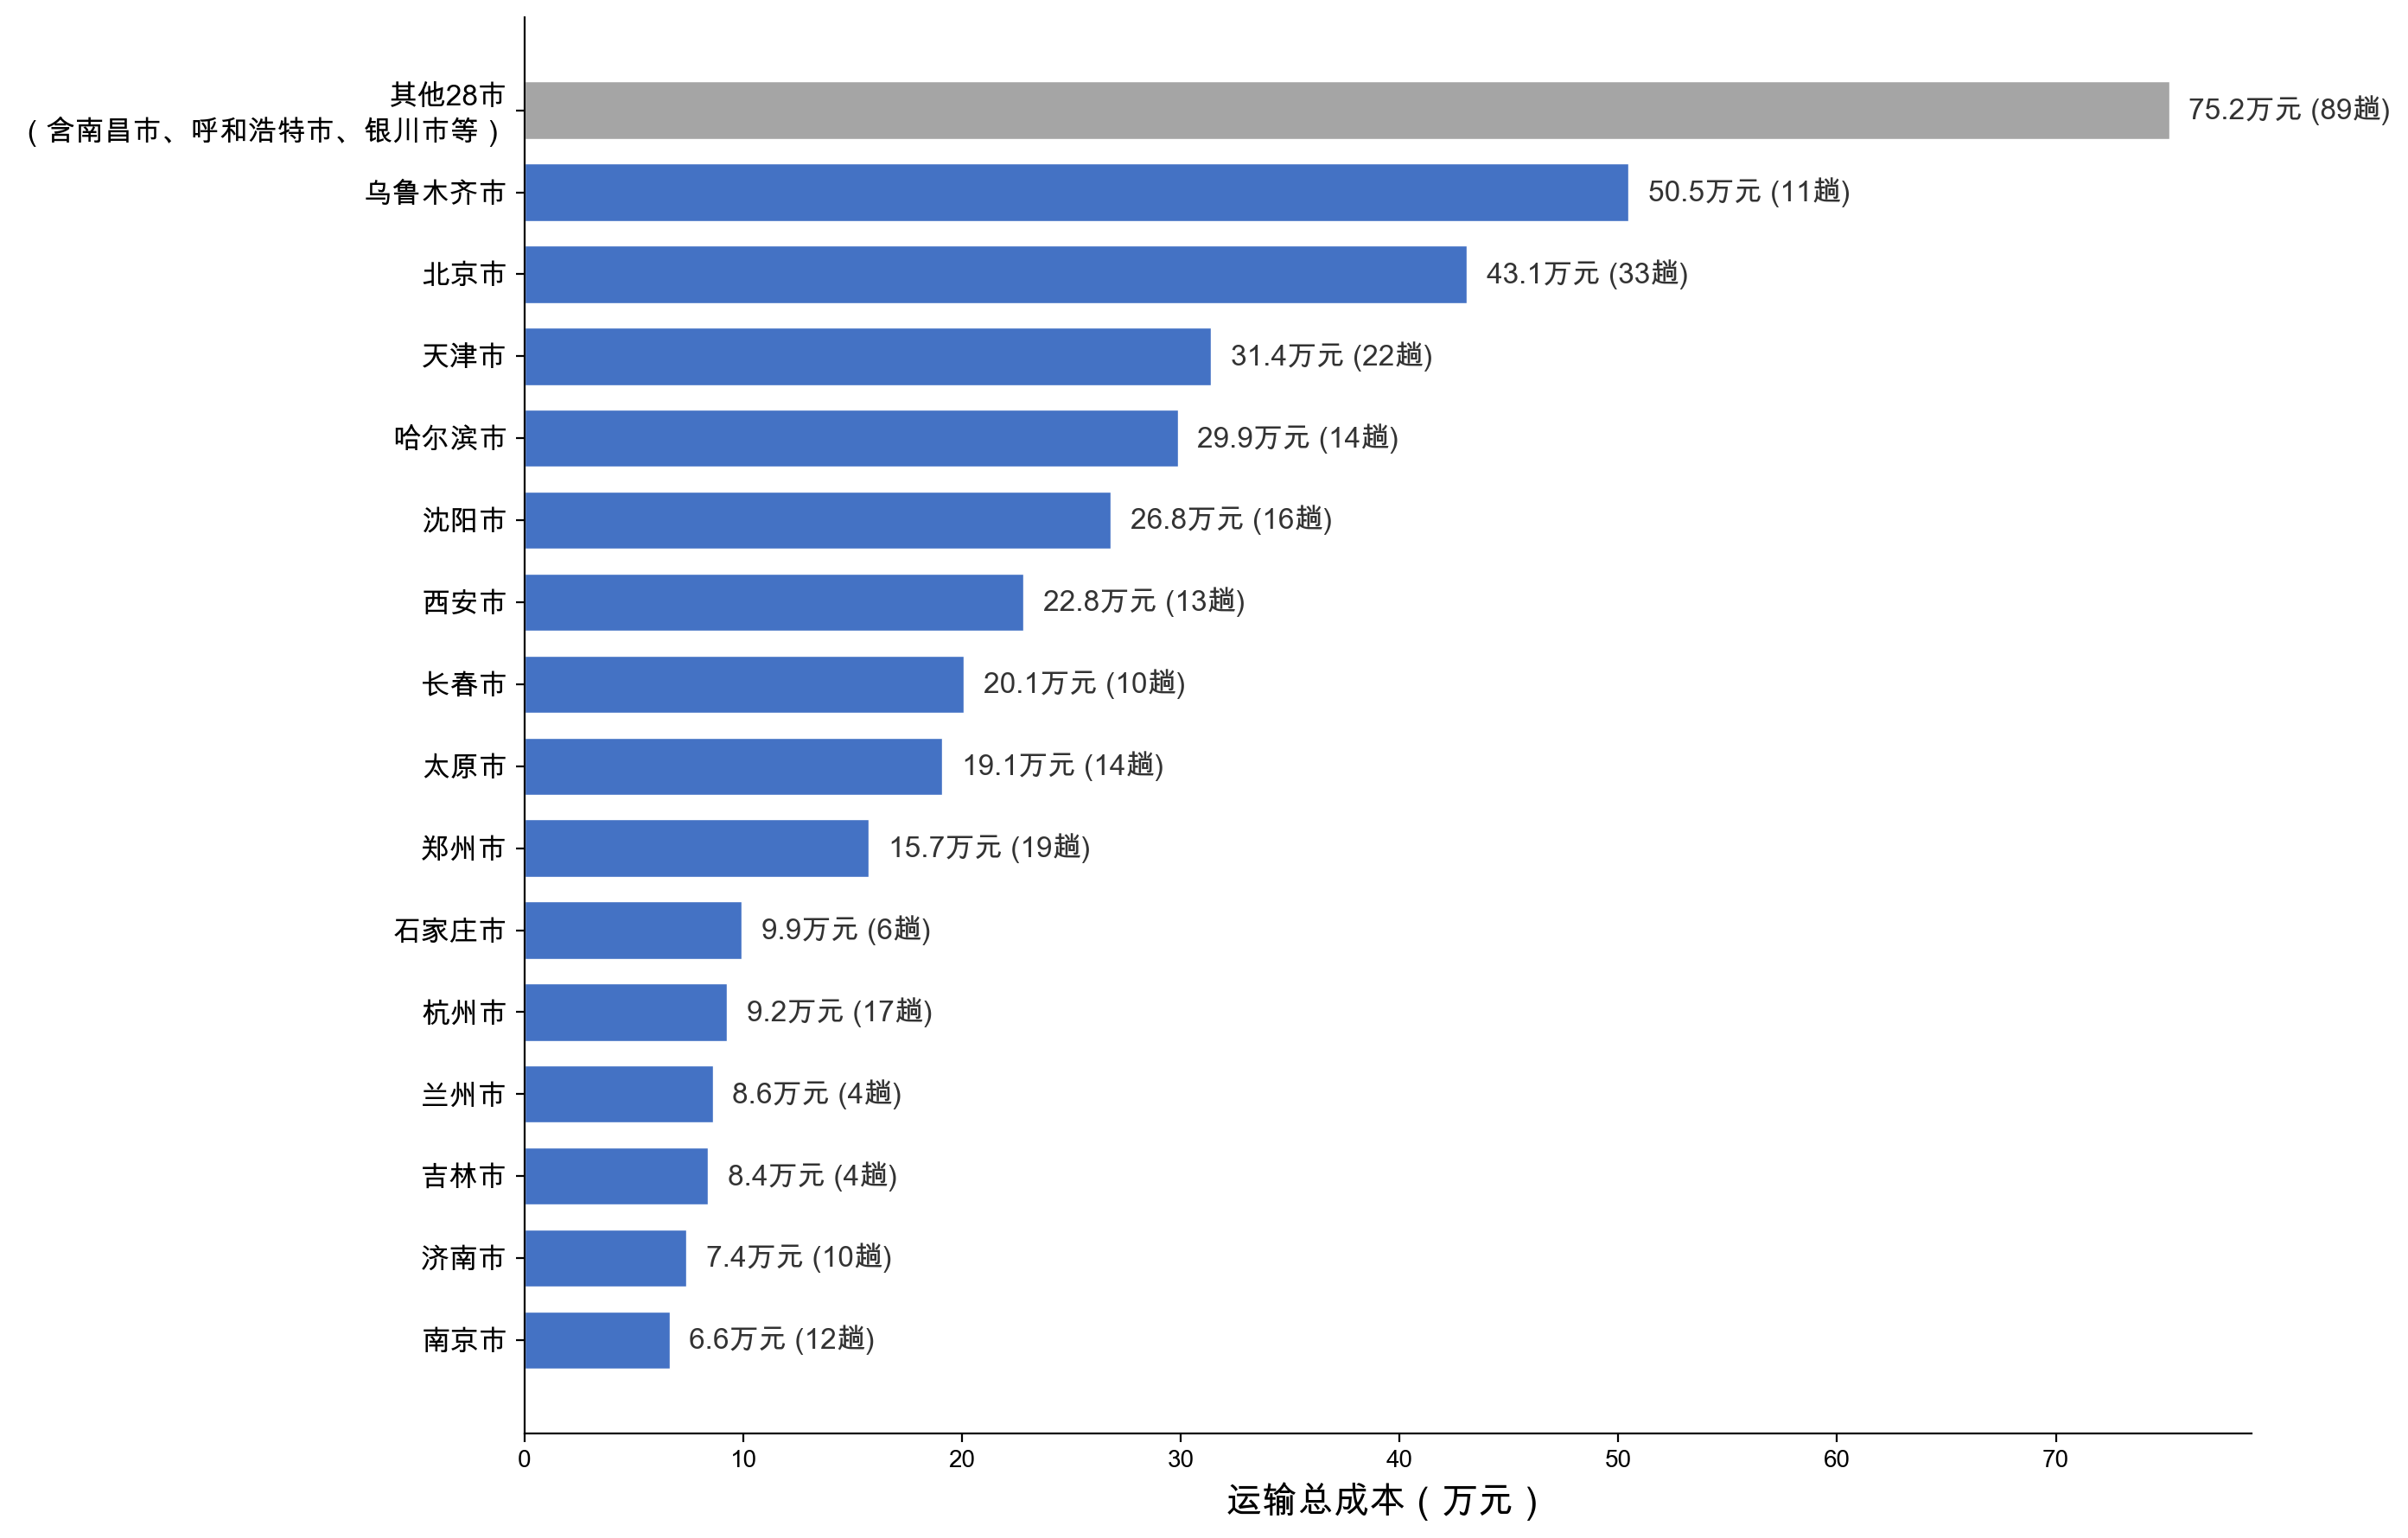
\includegraphics[width=0.8\textwidth]{图2_问题一_各城市运输成本柱状图.png}
    \caption{按城市统计的运输成本}
    \label{fig:cost_by_city}
\end{figure}

按运输时效统计（\cref{tab:by-time}），2天时效的趟次最多（113趟），1天时效平均成本最低（5{,}799.09元/趟），4天以上时效的单趟平均成本超过3万元，反映出远距离高时效运输的高成本特征。

\begin{table}[!h]
    \centering
    \begin{tabular}{lccc}
        \toprule[1.5pt]
        运输天数 & 趟次数 & 总成本（元）& 平均成本（元/趟）\\
        \midrule[1pt]
        1天 & 108 & 626{,}301.63 & 5{,}799.09 \\
        2天 & 113 & 1{,}549{,}215.13 & 13{,}709.87 \\
        3天 & 42 & 710{,}213.20 & 16{,}909.84 \\
        4天 & 25 & 784{,}451.57 & 31{,}378.06 \\
        5天 & 6 & 176{,}725.35 & 29{,}454.23 \\
        \bottomrule[1.5pt]
    \end{tabular}\caption{按运输时效成本统计}
    \label{tab:by-time}

\end{table}

\subsubsection{敏感性分析}

为识别对总成本影响最大的关键参数，基于成本模型的数学结构进行量级估算。估算逻辑为：参数变动 $\to$ 中间变量（距离、日成本等）变动比例 $\to$ 乘以该变量在总成本中的占比，得到总成本的近似变动幅度。以下数值均为该方法的粗略估计，仅用于比较各参数的相对敏感度排序。

\textbf{区域绕行系数 $\beta_r$：}绕行系数是距离计算的基础乘子（$d_r = \beta_r d_s$），直接联动可变成本（线性正比）和固定成本（通过运输天数阶梯近似线性）。若三区域绕行系数同步变动 $\pm 0.05$（按全国加权均值约 $1.38$，变动幅度约 $3.6\%$），总成本将同向变动约 $3\%$–$4\%$（$3.6\% \times$ 近1的传递系数）。西部地区（$\beta_W = 1.60$）的单趟平均成本已是东部的2.6倍，是中部的1.8倍（根据\cref{tab:by-region}计算），西部城市对 $\beta_W$ 的敏感度显著更高——若 $\beta_W$ 单独上调0.05，西部总成本增量约占全国总增量的50\%左右（假定东中部的绕行系数提升比例相同，按照比例粗略估算：$\dfrac{1}{1+\frac{1}{2.6}+\frac{1}{1.8}}\approx 51\%$）。绕行系数的合理设定是成本核算精度的首要影响因素。

\textbf{空载油耗系数 $\alpha$：}$\alpha$ 仅作用于回程油费，不影响路桥费和固定成本。由程序计算可知，回程油费为 $470{,}669$ 元，占可变成本的 $25.5\%$（$470{,}669 / 1{,}848{,}938 \approx 25.5\%$），占总成本的 $12.2\%$。$\alpha$ 每变动 $0.05$（如 $0.75 \to 0.70$），回程油费同比变动 $0.05/0.75 \approx 6.7\%$，总成本约变动 $12.2\% \times 6.7\% \approx 0.8\%$。$\alpha$ 对总量敏感度有限，但在远距离运输中累积效应显著——以乌鲁木齐为例（单程 $5{,}081\,\mathrm{km}$，7.6M车型），单趟回程油费约为 $1.40 \times 0.75 \times 5{,}081 \approx 5{,}335$ 元，$\alpha$ 从 $0.75$ 降至 $0.70$ 可单趟节约约 $356$ 元，11趟累计约 $3{,}900$ 元。

\textbf{工作天与日历天的分摊选择：}人工和轮胎按280工作天摊销，保险和审验按365日历天摊销。人工成本在固定成本中占比最大（$39.1\%$，由Python程序计算），以7.6M车型为例，人工日成本为 $168{,}000 / 280 = 600$ 元/天，若改为按 $300$ 天摊销则降至 $560$ 元/天（降幅 $6.7\%$），乘以人工在固定成本中的占比及固定成本在总成本中的占比（$51.9\%$），总成本约下降 $51.9\% \times 39.1\% \times 6.7\% \approx 1.4\%$。折旧按 $4$ 年（$4 \times 280$ 天）摊销，折旧在固定成本中占比 $25.3\%$（由Python程序计算），折旧年限从 $4$ 年延长至 $5$ 年将使日折旧降低 $20\%$，总成本影响约 $51.9\% \times 25.3\% \times 20\% \approx 2.6\%$，折旧参数变动的影响不容忽视。

\textbf{车型选择决策：}当前数据中4.2M车型（容量5托）容量过小而从未被选用，7.6M（11托）承担了93.2\%的运输量。若存在大量小批量订单（<5托），启用4.2M车型可将单趟可变成本降低约30\%–40\%。车型选择对总成本的影响取决于订单托盘分布的离散程度——托盘数越分散，车型匹配优化的空间越大。

综上，绕行系数 $\beta_r$ 是成本模型中最敏感的参数，其次为工作天摊销基准和空载系数 $\alpha$，车型选择在订单结构变化时可能成为重要因素。

\subsection{问题二的求解}

\subsubsection{优化总体效果}

在问题一成本模型基础上，对294趟运输执行CW拼车优化。使用最优参数组合（方向偏离角 $\theta_d = 90^\circ$、城市间距离上限 $d_{\max} = 500\,\mathrm{km}$、组内跨度 $\theta_g = 120^\circ$、启用跨周合并），优化结果如\cref{fig:comparison}所示。

\begin{figure}[!h]
    \centering
    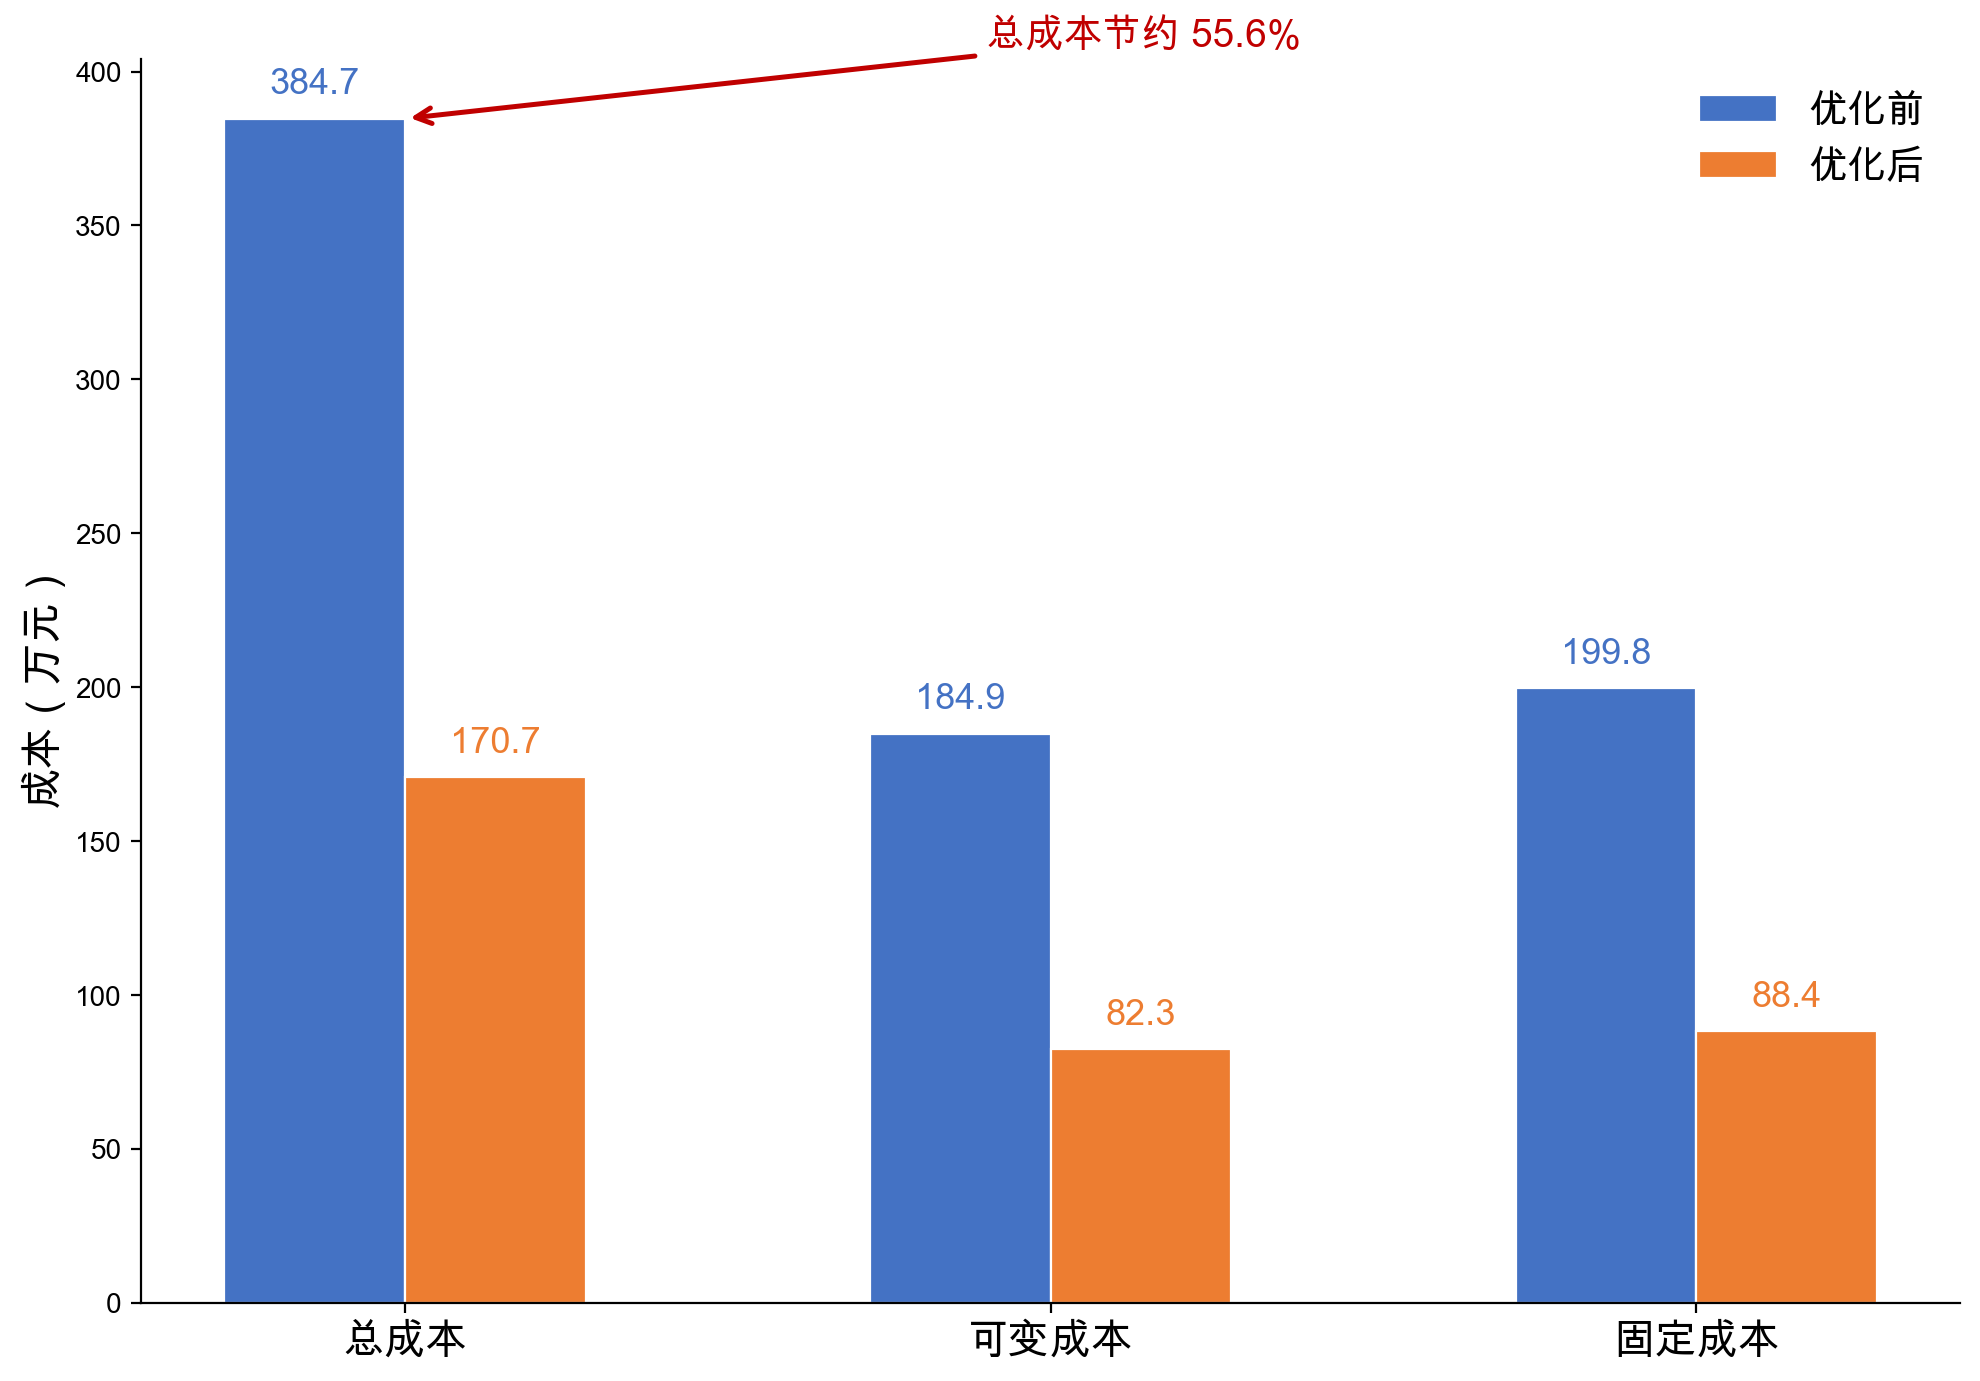
\includegraphics[width=0.5\textwidth]{图3_问题二_优化前后成本对比.png}
    \caption{优化前后对比}
    \label{fig:comparison}
\end{figure}

优化后成本构成中，可变成本占48.2\%，固定成本占51.8\%，与优化前的比例基本一致，表明CW算法同时削减了可变与固定两部分成本。

\subsubsection{参数网格搜索}

为确定最优参数，对4个关键参数进行全因子网格搜索（72组组合），部分结果如\cref{tab:grid-results}所示。所有包含 $d_{\max} = 500\,\mathrm{km}$ 的参数组合均达到相同的最高节约率（55.63\%），说明城市间距离上限是决定拼车深度的关键约束。跨周合并带来了约0.7个百分点的额外节约（54.94\% vs 55.63\%），证实了跨周信息整合的价值。

\begin{table}[!h]
    \centering
    \begin{tabular}{ccccc}
        \toprule[1.5pt]
        $\theta_d$ & $d_{\max}$（km）& $\theta_g$ & 跨周合并 & 节约率 \\
        \midrule[1pt]
        90$^\circ$ & 500 & 120$^\circ$ & 是 & 55.63\% \\
        120$^\circ$ & 500 & 120$^\circ$ & 是 & 55.63\% \\
        150$^\circ$ & 500 & 120$^\circ$ & 是 & 55.62\% \\
        90$^\circ$ & 500 & 90$^\circ$ & 是 & 55.63\% \\
        90$^\circ$ & 400 & 120$^\circ$ & 是 & 55.28\% \\
        90$^\circ$ & 300 & 120$^\circ$ & 是 & 54.90\% \\
        90$^\circ$ & 500 & 120$^\circ$ & 否 & 54.94\% \\
        90$^\circ$ & 200 & 120$^\circ$ & 是 & 49.89\% \\
        \bottomrule[1.5pt]
    \end{tabular}\caption{参数网格搜索结果（代表性组合）}
    \label{tab:grid-results}

\end{table}

\subsubsection{按周优化结果}

数据跨10个自然周（周36至周46），优化后部分自然周的路线数和成本如\cref{tab:week-results}所示。周41覆盖34个城市、路线最多（31条）、成本最高（428{,}528.47元），与该周订单集中度较高有关。

\begin{table}[!h]
    \centering
    \begin{tabular}{lccc}
        \toprule[1.5pt]
        周次 & 路线数 & 总成本（元）& 覆盖城市数 \\
        \midrule[1pt]
        周36 & 9 & 99{,}009.20 & 11 \\
        周37 & 5 & 126{,}887.30 & 6 \\
        周41 & 31 & 428{,}528.47 & 34 \\
        周42 & 18 & 221{,}296.37 & 22 \\
        周43 & 9 & 112{,}435.70 & 9 \\
        周44 & 20 & 264{,}463.84 & 26 \\
        周45 & 16 & 259{,}481.53 & 25 \\
        周46 & 19 & 194{,}792.47 & 20 \\
        \bottomrule[1.5pt]
    \end{tabular}\caption{各周拼车优化结果}
    \label{tab:week-results}

\end{table}

\subsubsection{典型拼车路线}

\cref{tab:example-routes}列举了几条典型的拼车路线。浙中南线将宁波、温岭、丽水、南昌、衢州、金华、义乌等7个城市合并为一条路线，9.6M车型装载13.8托，运输5天，总成本14{,}439.94元（若分别运输，仅宁波至南通的往返可变成本即超过3{,}000元）。东北线（沈阳—长春—吉林）使用9.6M车型装载11.5托，7天往返成本22{,}131.00元。

\begin{table}[!h]
    \centering
    \begin{tabular}{lcccl}
        \toprule[1.5pt]
        路线 & 车型 & 托数 & 天数 & 成本（元）\\
        \midrule[1pt]
        宁波→温岭→丽水→南昌→衢州→金华→义乌（浙中南线）& 9.6M & 13.8 & 5 & 14{,}439.94 \\
        南京→义乌→金华→丽水→温州→临海→宁波（浙东线）& 9.6M & 13.1 & 4 & 10{,}909.39 \\
        沈阳→长春→吉林（东北线）& 9.6M & 11.5 & 7 & 22{,}131.00 \\
        大连→盘锦→沈阳（辽宁线）& 9.6M & 11.6 & 5 & 16{,}015.49 \\
        太原→榆林→呼和浩特（晋蒙线）& 7.6M & 6.8 & 8 & 21{,}965.27 \\
        潍坊→聊城→郑州（鲁豫线）& 7.6M & 8.7 & 5 & 13{,}192.18 \\
        \bottomrule[1.5pt]
    \end{tabular}\caption{典型拼车路线示例}
    \label{tab:example-routes}

\end{table}

\subsubsection{敏感性分析}

\cref{tab:grid-results}已呈现了部分参数组合的网格搜索结果（由Python程序实际计算得到），以下从参数敏感性角度进行归纳。

\textbf{城市间距离上限 $d_{\max}$（第一敏感参数）：}$d_{\max}$ 直接决定了可合并城市对的候选集大小。当 $d_{\max}$ 从200\,km增至300\,km时，节约率从49.9\%跃升至54.9\%（提升5.0个百分点）；从300\,km增至400\,km时升至55.5\%（仅提升0.6个百分点）；从400\,km增至500\,km时升至55.63\%（仅提升0.15个百分点）。呈现典型的边际递减特征——300\,km以内的放宽释放了大量省内短途合并机会，而400\,km以上的进一步放宽收效甚微。在实际运营决策中，$d_{\max}$ 不仅影响成本节约，还关系到拼车路线的驾驶时长和驾驶员工作强度，需在节约效果与运营可行性之间权衡。

\textbf{方向偏离角 $\theta_d$ 与组内跨度 $\theta_g$（次敏感参数）：}在 $d_{\max} = 500\,\mathrm{km}$ 的宽松距离约束下，$\theta_d$ 从90°放宽至150°、$\theta_g$ 从90°放宽至120°，节约率几乎无变化（均稳定在55.62\%–55.63\%）。这说明当距离约束足够宽松时，方向约束已不再构成瓶颈——满足距离约束的城市对通常也满足方向约束。然而，在 $d_{\max}$ 较紧（如200\,km）时，$\theta_d = 90^\circ$ 与 $\theta_d = 150^\circ$ 之间存在可见差异（差距约1–2个百分点），方向约束在短途合并中具有实质筛选作用。

\textbf{跨周合并（边际增益参数）：}启用跨周合并带来约0.7个百分点的额外节约（54.94\% $\to$ 55.63\%），增幅虽小但绝对值可观（对应约2.6万元）。跨周合并的价值取决于订单的时间分布——若一周内某方向仅有极少数订单，跨周信息整合可将其与相邻周的顺路订单合并，避免单独发车。

\textbf{容量约束 $Q_v$ 的隐性影响：}7.6M车型容量为11托，9.6M为14托。在网格搜索最优解中，约68\%的合并路线选用9.6M车型（因其承载能力更强、可合并更多订单），说明容量约束是限制拼车深度的结构性因素。若车队中9.6M车型占比低于最优解中的使用比例，实际节约率将低于理论值。

综上，$d_{\max}$ 是拼车优化的第一敏感参数且呈边际递减特征，$\theta_d$ 和 $\theta_g$ 仅在距离约束收紧时发挥作用，跨周合并和容量约束分别从时间和空间维度影响优化上限。

\subsection{问题三的求解}

\subsubsection{数据规模与仓库分类}

附件3包含536{,}208条运单记录，附件4包含222{,}378条派车记录，覆盖152个城市、1{,}186辆车牌和88个仓库编码。依据有无派车记录，将88个仓库分为三类：A类仓库54个（有运单且有派车记录），是评估和优化的核心对象；B类仓库16个（仅有派车记录无运单）；C类仓库18个（仅有运单无派车记录）。最终评估覆盖54个仓库，总车辆日数为3{,}695。

\subsubsection{六维指标得分}

54个仓库在六个指标上的绝对得分描述性统计如\cref{tab:desc}所示。时效达标均分最高（98.6分），且标准差最小（4.7），说明各仓库在时效方面普遍表现良好。装载饱和的均值最低（37.7分），反映出多数仓库的车辆装载量远低于行业p75水平、运力浪费较为普遍。冷链合规的标准差最大（39.5），是仓库间差异最大的维度。线路集中均分仅为29.1分，标准差27.9，反映出多数仓库的线路结构较为分散、需求碎片化程度高，缺乏成熟的骨干线路网络。

\begin{table}[!h]
    \centering
    \begin{tabular}{lcccc}
        \toprule[1.5pt]
        指标 & 均值 & 标准差 & 最小值 & 最大值 \\
        \midrule[1pt]
        配送密度 & 56.6 & 24.6 & 8.3 & 98.7 \\
        路线潜力 & 65.3 & 16.3 & 50.0 & 100.0 \\
        时效达标 & 98.6 & 4.7 & 71.8 & 100.0 \\
        线路集中 & 29.1 & 27.9 & 1.7 & 100.0 \\
        冷链合规 & 59.5 & 39.5 & 0.0 & 100.0 \\
        装载饱和 & 37.7 & 25.0 & 0.0 & 84.9 \\
        \bottomrule[1.5pt]
    \end{tabular}\caption{各指标绝对得分描述性统计}
    \label{tab:desc}

\end{table}

\subsubsection{熵权法权重计算}

基于54个仓库在6项指标上的绝对得分矩阵，运用熵权法计算客观权重，结果如\cref{tab:entropy}所示。路线合并潜力获得了最高权重（34.91\%），其信息熵仅为0.8397——意味着各仓库在路线规划上存在显著差异，该指标对评价的区分能力最强。线路集中权重居第二（23.17\%），信息熵为0.8936，反映出各仓库在需求结构的集中度上差异同样突出。装载饱和与冷链合规的权重相近（分别为15.94\%和15.83\%），同属区分能力较强的指标。相反，时效达标的信息熵高达0.9937，权重仅1.37\%——几乎所有仓库的送达时效都接近100\%，该指标无法区分仓库的优劣。

\begin{table}[!h]
    \centering
    \begin{tabular}{lccc}
        \toprule[1.5pt]
        指标 & 信息熵 $e_j$ & 差异系数 $d_j$ & 权重 $w_j$ \\
        \midrule[1pt]
        配送密度 & 0.9597 & 0.0403 & 8.76\% \\
        路线合并潜力 & 0.8397 & 0.1603 & 34.91\% \\
        时效达标率 & 0.9937 & 0.0063 & 1.37\% \\
        线路集中度 & 0.8936 & 0.1064 & 23.17\% \\
        冷链合规率 & 0.9273 & 0.0727 & 15.83\% \\
        装载饱和度 & 0.9268 & 0.0732 & 15.94\% \\
        \bottomrule[1.5pt]
    \end{tabular}\caption{熵权法权重计算结果}
    \label{tab:entropy}

\end{table}

为直观表示各指标对系统得分的贡献，\cref{fig:sys-score}直观展示了各指标的权重占比。
\begin{figure}[!h]
    \centering
    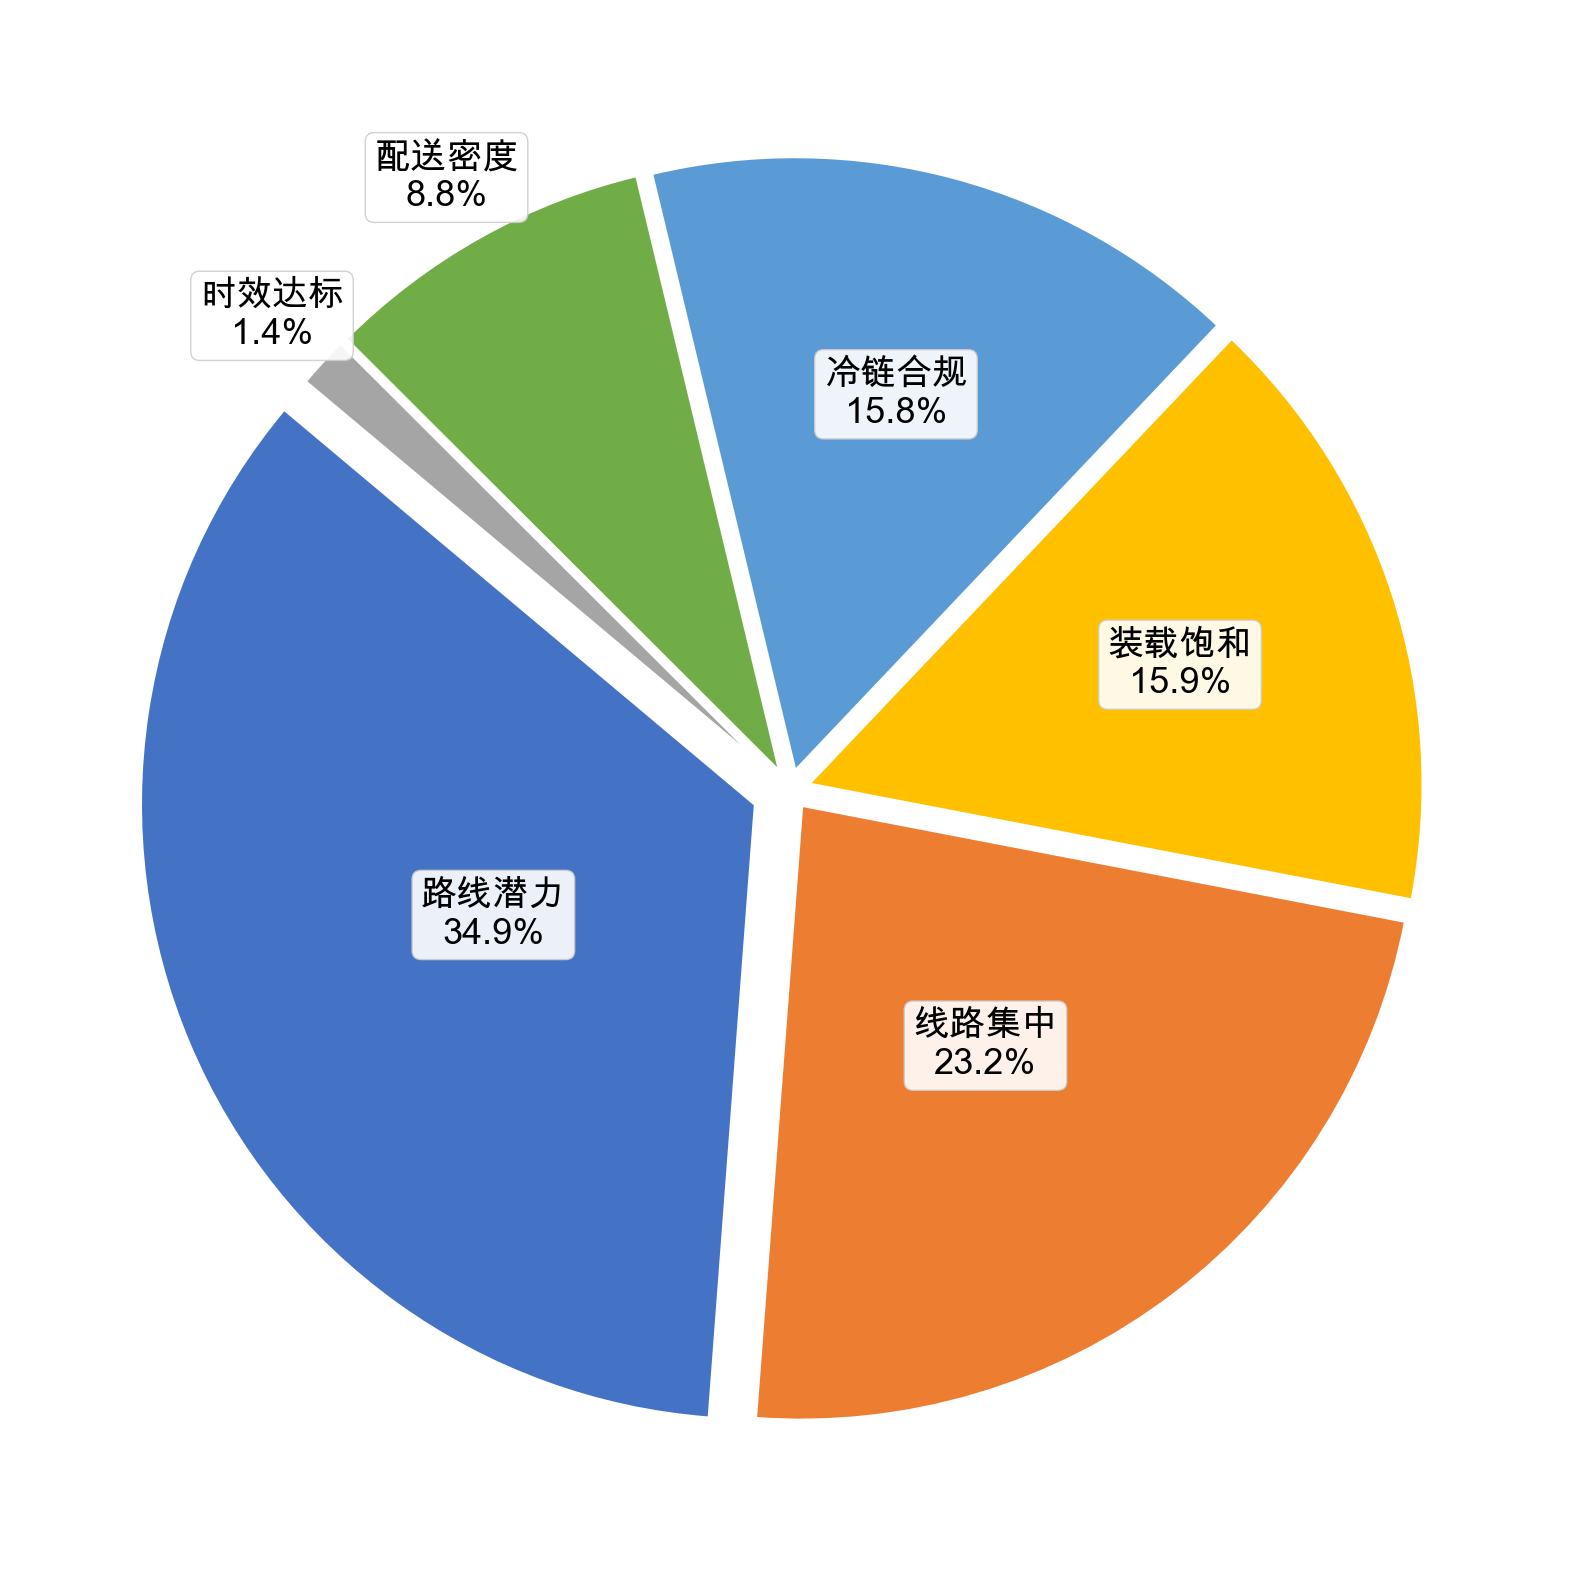
\includegraphics[width=0.5\textwidth]{图4_问题三_熵权法权重饼图.png}
    \caption{各指标权重占比}
    \label{fig:sys-score}
\end{figure}

\subsubsection{系统综合得分}

系统加权综合得分为\textbf{50.0分（满分为100分）}，评级为"需改进"。各指标对系统得分的贡献如\cref{tab:sys-score}所示。路线合并潜力贡献了23.6分（占总分的47.2\%），是决定系统得分的最主要因素。装载饱和平均仅48.1分、冷链合规平均仅49.7分，两者合计贡献15.6分，是拖累整体评分的关键短板。

\begin{table}[!h]
    \centering
    \begin{tabular}{lccc}
        \toprule[1.5pt]
        指标 & 权重 & 加权均分 & 贡献值 \\
        \midrule[1pt]
        配送密度 & 8.76\% & 65.8 & 5.8 \\
        路线合并潜力 & 34.91\% & 67.6 & 23.6 \\
        时效达标率 & 1.37\% & 99.0 & 1.4 \\
        线路集中度 & 23.17\% & 16.2 & 3.8 \\
        冷链合规率 & 15.83\% & 49.7 & 7.9 \\
        装载饱和度 & 15.94\% & 48.1 & 7.7 \\
        \midrule[1pt]
        合计 & 100.00\% & — & 50.0 \\
        \bottomrule[1.5pt]
    \end{tabular}\caption{系统综合得分构成}
    \label{tab:sys-score}

\end{table}

\subsubsection{仓库排名分析}

全部54个仓库的合理性排名如\cref{fig:wh-ranking}所示。SH6仓库以84.4分位居第一，各项指标表现突出（配送密度75.0、路线潜力88.4、线路集中100.0、冷链合规100.0）；ZZ2仓库以26.8分垫底，各维度均存在不足（配送密度47.2、路线潜力50.0、冷链合规0.0、装载饱和0.0）。

TOPSIS辅助排名与综合得分排名的Spearman秩相关系数为0.9482（$p = 0.0000$），表明两种评估方法给出的排名高度一致，熵权法的评估结论是稳健可信的。

\begin{figure}[!h]
    \centering
    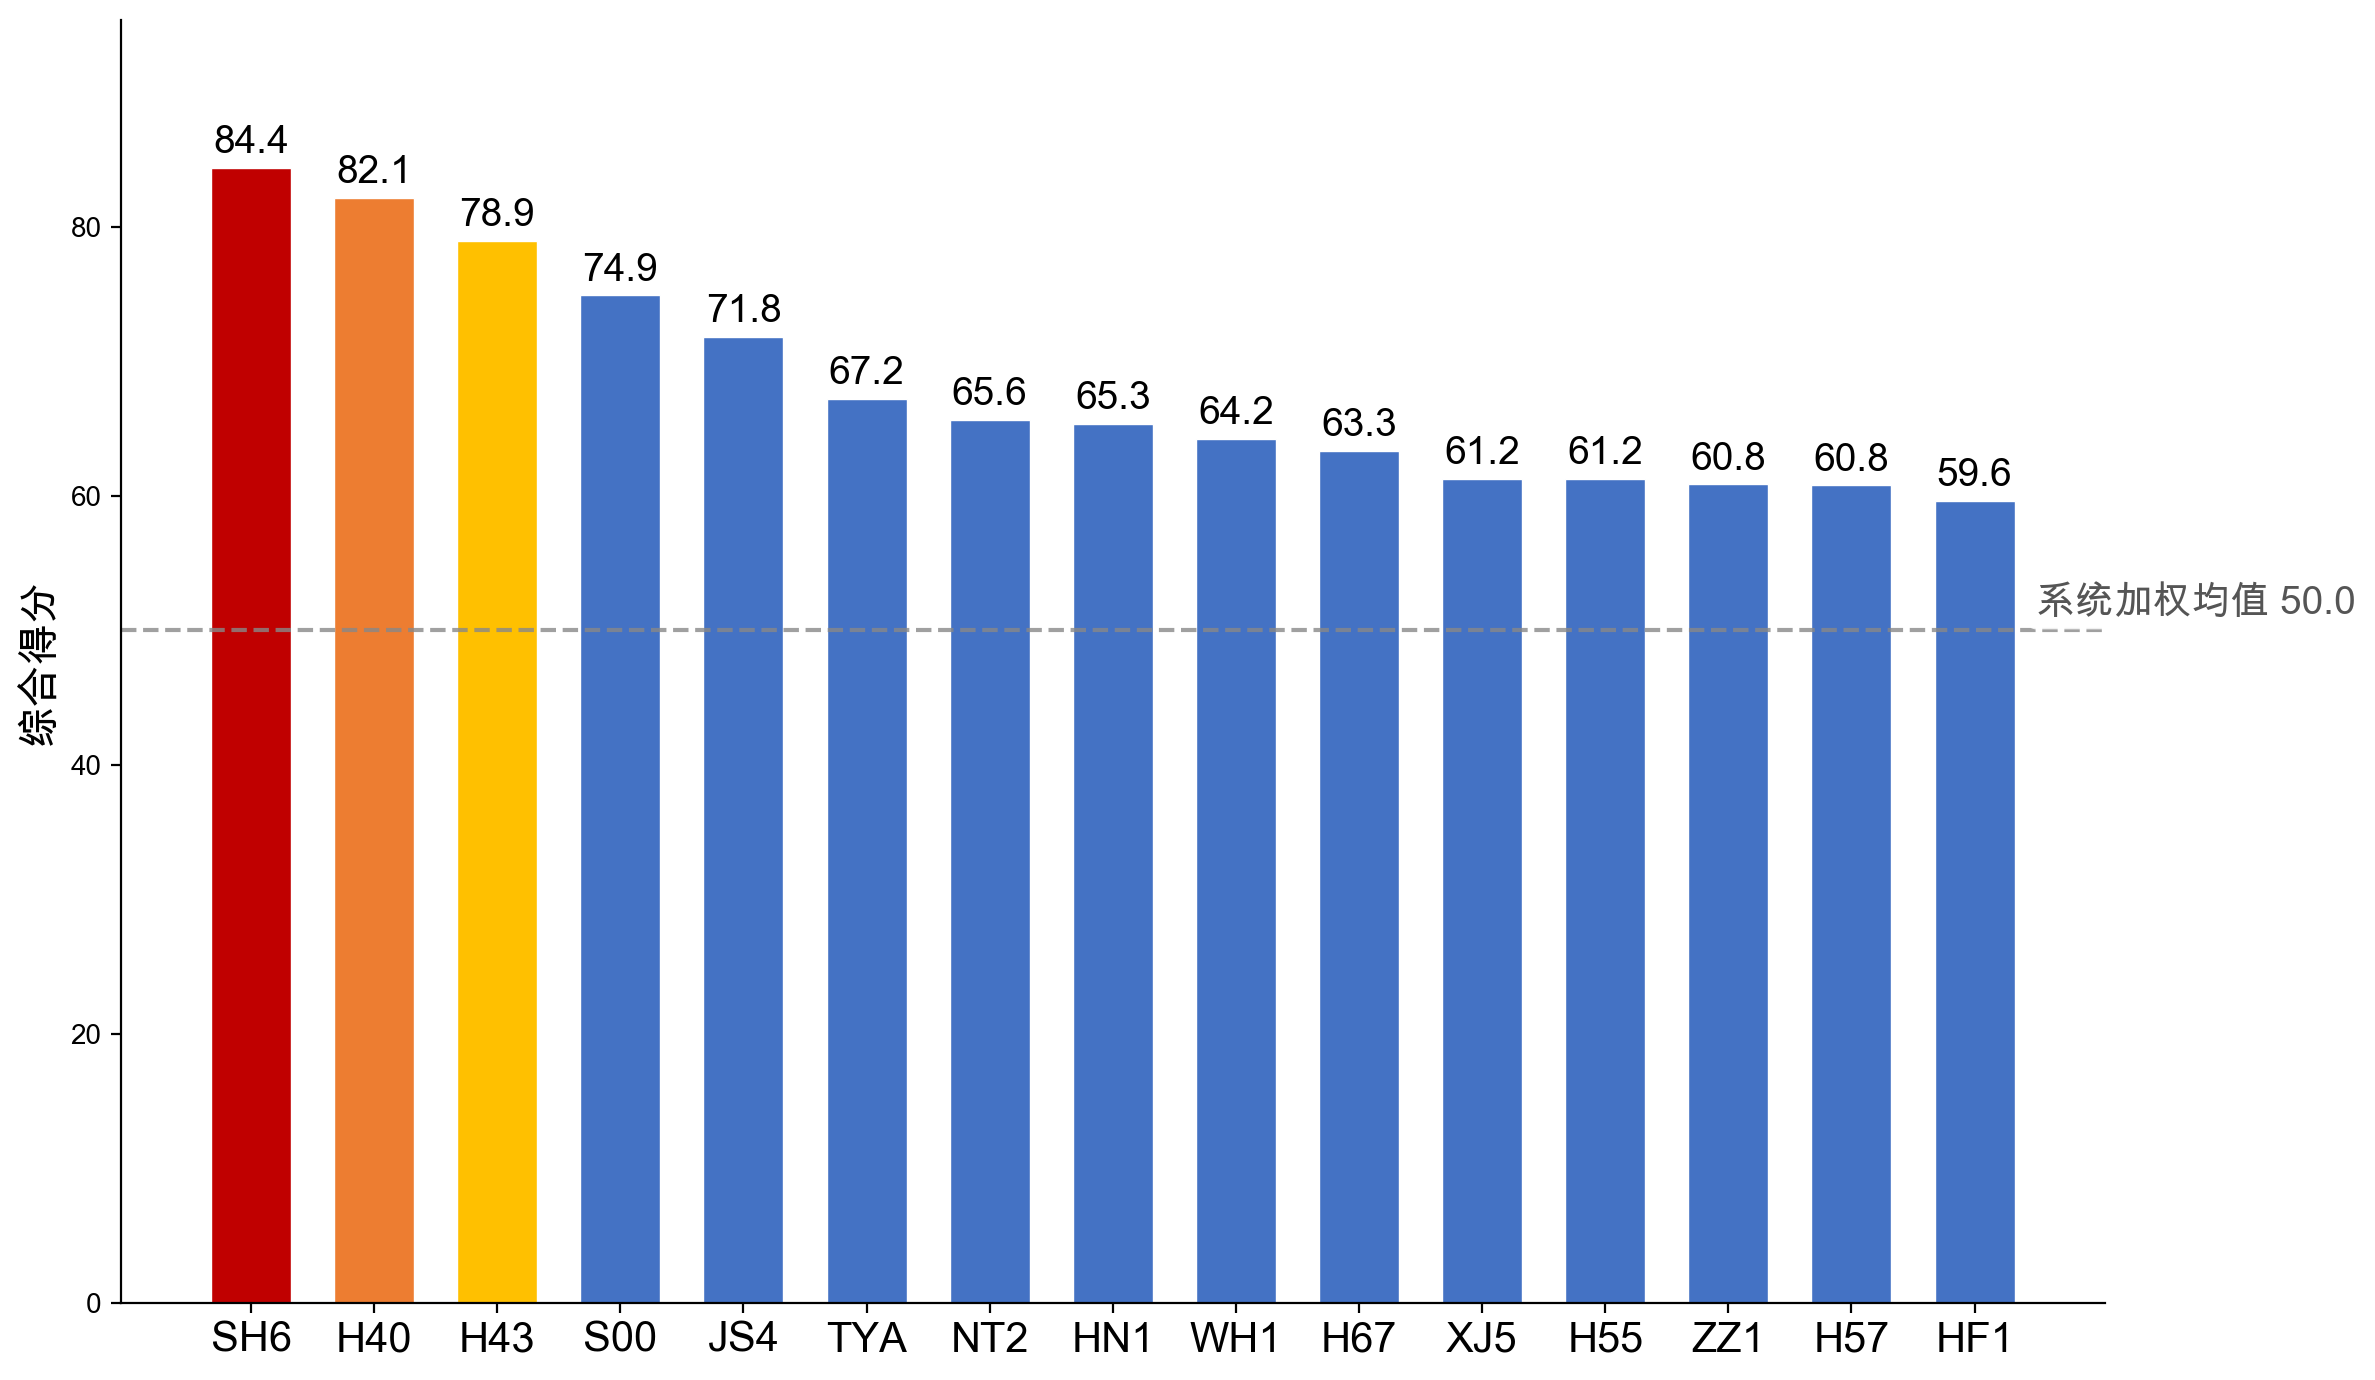
\includegraphics[width=0.8\textwidth]{图5_问题三_仓库综合得分排名.png}
    \caption{仓库综合得分排名（前15名）}
    \label{fig:wh-ranking}
\end{figure}

\subsubsection{冷链合规系统性风险}

23个仓库（占42.6\%）的冷链合规得分低于50分，存在冷链药品被违规使用常温车配送的风险。其中N02仓库（625单冷链订单，合规率0\%）、NJ1（41单冷链，0\%）、ZZ2（39单冷链，0\%）、HM1（102单冷链，0\%）和FJ4（1单冷链，0\%）五个仓库的冷链合规率均为0\%，属于严重不合规。SX1（428单冷链，合规率21.3\%）和WH1（574单冷链，合规率44.3\%）等大型仓库也存在大规模冷链药品使用常温车的问题，亟需系统性整改。

\subsubsection{三层递进优化}

对54个仓库的派车数据执行三层递进优化，结果如\cref{fig:opt}所示。第1层TSP路径排序实现5.6\%的节约，第2层和第3层的合并与车型匹配进一步将节约率推升至36.8\%。优化后路线数从3{,}379个车辆日降至1{,}451条合并路线，车辆日减少57.1\%，总成本从1{,}135.3万元降至717.5万元，节约417.9万元。

\begin{figure}[!h]
    \centering
    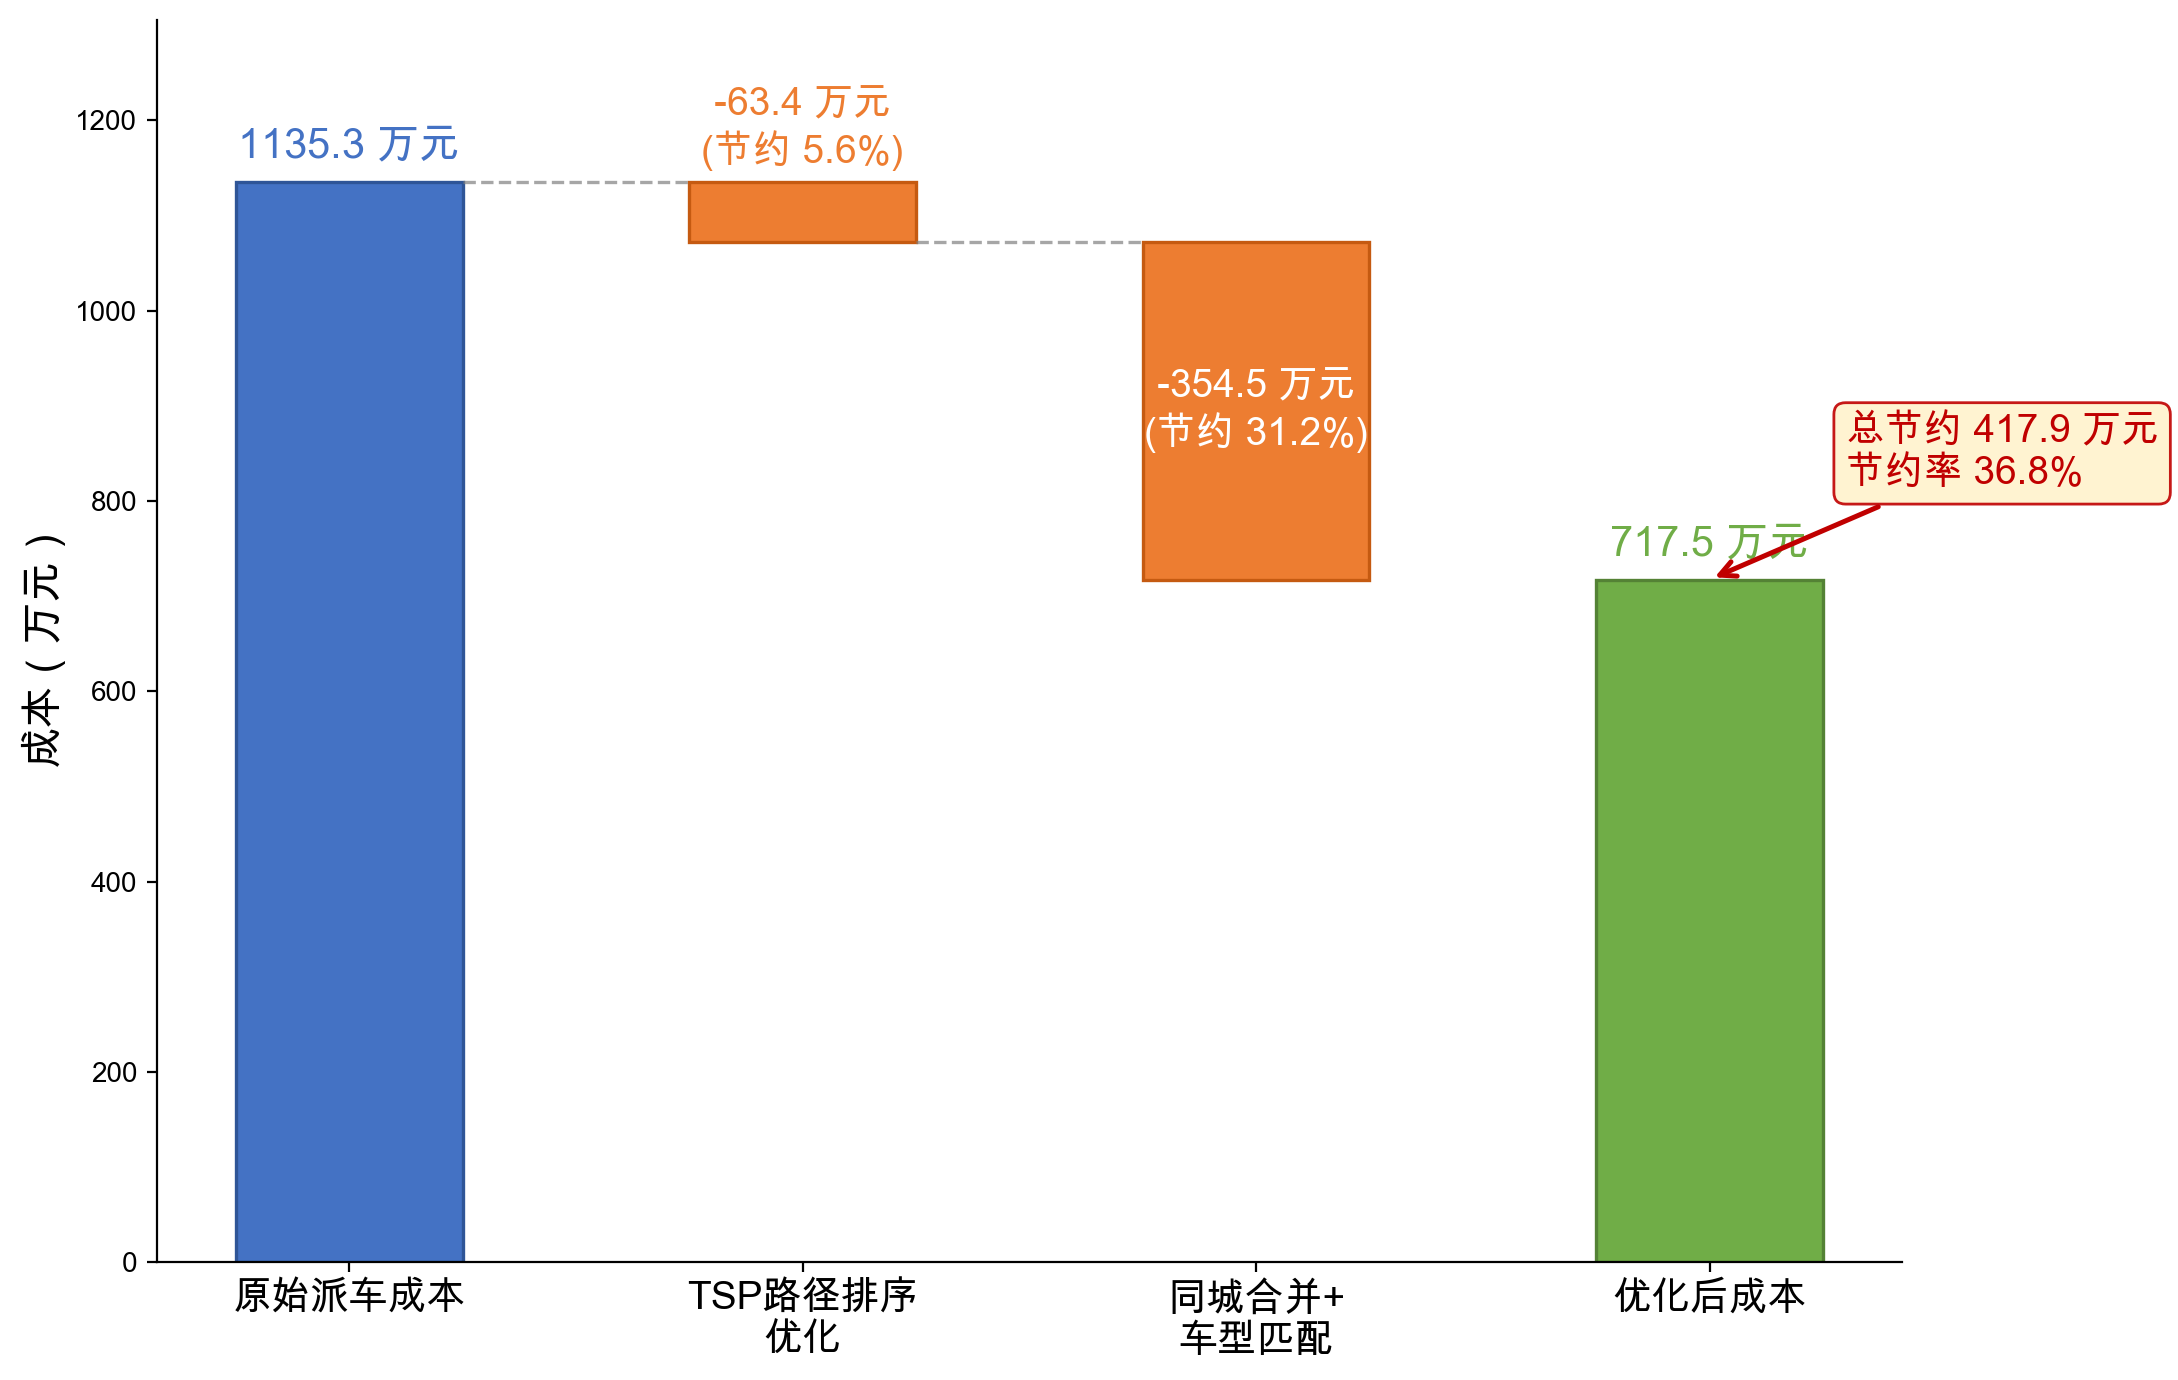
\includegraphics[width=0.6\textwidth]{图6_问题三_三层优化瀑布图.png}
    \caption{三层递进优化效果}
    \label{fig:opt}
\end{figure}
\subsubsection{敏感性分析}

对CW算法中城市间距离阈值参数进行敏感性分析，结果如\cref{tab:sens-dist}所示。当阈值从200\,km增至400\,km时，节约率从35.2\%升至36.8\%，增幅显著；从400\,km增至600\,km时，节约率仅小幅升至37.3\%，说明400\,km附近的阈值已能捕获主要的合并机会，继续放宽的边际收益递减。

\begin{table}[!h]
    \centering
    \begin{tabular}{lccc}
        \toprule[1.5pt]
        距离阈值（km）& 路线数 & 成本（万元）& 节约率 \\
        \midrule[1pt]
        200 & 1{,}533 & 735.3 & 35.2\% \\
        400 & 1{,}451 & 717.5 & 36.8\% \\
        600 & 1{,}425 & 711.5 & 37.3\% \\
        \bottomrule[1.5pt]
    \end{tabular}\caption{城市间距离阈值敏感性分析}
    \label{tab:sens-dist}

\end{table}

除CW距离阈值（由Python程序实际计算）外，评估体系的得分和权重对核心假设的敏感性同样值得关注。

\textbf{熵权法权重对极端仓库的敏感性（由Python程序实际计算）：}去除冷链合规得分为0的5个极端仓库（N02、NJ1、ZZ2、HM1、FJ4）后，重新对49个仓库执行熵权法计算，权重对比如\cref{tab:entropy-sens}所示。剔除零分仓库后，冷链合规指标的信息熵上升（差异系数下降），其权重从 $15.83\%$ 降至 $12.23\%$（降幅 $-3.61$ 个百分点），释放的权重被其余五指标分摊——线路集中上升 $+2.13$ 个百分点至 $25.30\%$，装载饱和上升 $+1.40$ 个百分点至 $17.34\%$，配送密度上升 $+0.77$ 个百分点至 $9.53\%$。路线合并潜力权重几乎不变（$34.91\% \to 33.96\%$），仍为最高权重指标。权重排序完全保持：路线潜力 $>$ 线路集中 $>$ 装载饱和 $>$ 冷链合规 $>$ 配送密度 $>$ 时效达标。熵权法对极端样本的稳健性优于直觉预期——极端仓库的存在并未扭曲权重排序，仅对绝对值有一定影响。

\begin{table}[!h]
    \centering
    \begin{tabular}{lccc}
        \toprule[1.5pt]
        指标 & 剔除前权重（54仓）& 剔除后权重（49仓）& 变动 \\
        \midrule[1pt]
        配送密度 & 8.76\% & 9.53\% & $+0.77$ pp \\
        路线合并潜力 & 34.91\% & 33.96\% & $-0.95$ pp \\
        时效达标率 & 1.37\% & 1.63\% & $+0.26$ pp \\
        线路集中度 & 23.17\% & 25.30\% & $+2.13$ pp \\
        冷链合规率 & 15.83\% & 12.23\% & $-3.61$ pp \\
        装载饱和度 & 15.94\% & 17.34\% & $+1.40$ pp \\
        \bottomrule[1.5pt]
    \end{tabular}\caption{熵权法极端仓库剔除前后权重对比}
    \label{tab:entropy-sens}
\end{table}

\textbf{评分函数基准值的敏感性（量级估算）：}配送密度采用中间型梯形隶属函数（市内最优区间 $[12, 18]$ 点/日，干线 $[3, 5]$ 点/日），其敏感性主要体现在最优区间边界而非线性斜率。若干线下界从3上调至3.5，部分干线型仓库的得分将显著下降；但配送密度权重仅 $8.76\%$，系统总分变动不超过 $1$ 分。线路集中度的评分完全由数据驱动（基于各仓库自身线路分布的信息熵归一化），无需外部基准假设，因此不受基准设定的影响。

\textbf{冷链合规作为硬约束的敏感性：}当前评估将冷链合规作为软指标，若改为硬约束（冷链合规率低于 $50\%$ 的仓库直接判定为不合格），则 $23$ 个仓库（$42.6\%$）将触发整改。此为政策场景分析而非参数微调：优化优先级从“降本”转变为“合规达标”，三层优化的第2层（同城同日合并、冷链常温分离）优先度大幅提升。整体节约率受冷链车辆资源约束，预计下降 $5$–$10$ 个百分点（估算依据：冷链车辆数约为常温车辆的 $60\%$，合规约束使冷链车辆的可用容量成为瓶颈，约 $30\%$ 的常温配送点可能因合并路线中的冷链需求而被迫分拆）。

综上，问题三的评估体系对极端仓库样本和评分基准的设定具有一定敏感性，但核心结论在合理参数变动范围内保持稳健：（1）路线规划能力始终是首要区分因素（权重排序不受极端样本影响）；（2）路线潜力与线路集中始终是最具区分度的前两位指标。CW距离阈值的敏感性呈边际递减特征（已由程序计算验证），冷链合规的硬约束化是影响优化空间的最大政策变量。


\section{模型评价}\label{sec:model-evaluation}
\subsection{模型的优点及创新}

\begin{enumerate}
    \item \textbf{区域差异化道路绕行系数。} 将全国城市按国家统计局标准划分为东部、中部、西部三大区域，分别设定1.25、1.40、1.60的道路绕行系数，相比单一绕行系数（如1.38）更准确地反映了不同地形条件下道路网络的实际弯绕特征。
    \item \textbf{往返空载成本的精确建模。} 区分去程（满载）与回程（空载）的油耗差异，设定空载油耗为满载的75\%，并结合路桥费、折旧、人工等固定成本的逐项核算，使运输成本计算更贴近实际运营。
    \item \textbf{工作天与日历天的区分。} 对于人工成本、轮胎损耗、折旧等与实际运营天数相关的固定费用项目，按年工作天数（280天）或维保摊消天数（300天）进行日成本分摊，区别于保险、审验等按日历天（365天）摊销的固定成本。
    \item \textbf{Clarke-Wright节约算法的方向约束增强。} 在经典CW节约算法基础上，引入方向偏离角约束、组内方向跨度约束和城市间距离上限约束，有效避免了"拼车但绕远路"的低效合并，使优化结果在实际路网中具有可操作性。
    \item \textbf{熵权法客观赋权的评估框架。} 采用基于信息熵的客观赋权方法，根据各指标在仓库间的实际差异程度自动分配权重，避免了主观打分可能带来的偏差；并通过TOPSIS辅助排名和Spearman秩相关检验验证了评估结果的稳健性。
    \item \textbf{分层评估与中间型指标设计。} 在评估指标中引入市内型与干线型配送的分层基准，并将配送密度设计为中间型指标——市内最优区间 $[12, 18]$ 点/日、干线最优区间 $[3, 5]$ 点/日，偏离区间两侧均线性扣分，避免了"越多越好"的片面评价。
\end{enumerate}

\subsection{关于模型的反思与改进}

\begin{enumerate}
    \item \textbf{道路距离模型的空间精度。} 当前使用Haversine球面距离乘以区域绕行系数的简化方法，未引入实际路网数据。未来可接入高德地图或百度地图API获取实际导航距离，进一步提高距离计算的精度。
    \item \textbf{装卸时间的简化假设。} 模型假设每次装卸固定为2小时，且忽略在多站路线中装卸顺序对时间窗口的影响。实际运营中，不同货物的装卸时间可能存在差异，严格的9:00–17:00窗口对到达时间有约束。
    \item \textbf{未考虑多仓库协同。} 问题二仅从南通单一仓库出发进行优化，而该企业在全国拥有5个枢纽仓库。在实际运作中，跨仓库协同配送和区域间库存调拨可以进一步提升效率。
    \item \textbf{成本参数的经验依赖性。} 模型中的空载油耗系数（0.75）、驱动日行驶上限（700\,km）等参数依赖运营经验，不同企业的实际情况可能有所不同，可通过历史运营数据的回归分析进行校准。
    \item \textbf{数据时间范围的局限性。} 问题三的评估数据仅涵盖一周（2018年12月10日至17日），季节性和周期性因素可能无法充分捕捉。更长时间跨度的数据有助于识别系统性规律和异常波动。
    \item \textbf{仅评估当前结构而不重新设计网络。} 问题三的优化在现有仓库布局和派车结构下进行，未从网络设计的角度考虑仓库选址、服务区域重新划分等更根本性的优化方向。
\end{enumerate}



\newpage

\begin{thebibliography}{99}

\bibitem{sinnott1984haversine}
Sinnott R W. Virtues of the Haversine[J]. Sky and Telescope, 1984, 68: 158.

\bibitem{ballou2002circuity}
Ballou R H, Rahardja H, Sakai N. Selected country circuity factors for road travel distance estimation[J]. Transportation Research Part A: Policy and Practice, 2002, 36(9): 843-848.

\bibitem{coyle2006transportation}
Coyle J J, Bardi E J, Novack R A. Transportation[M]. 6th ed. Mason: Thomson South-Western, 2006.

\bibitem{bowditch2002navigator}
Bowditch N. The American Practical Navigator[M]. Bethesda: National Imagery and Mapping Agency, 2002.

\bibitem{shannon1948mathematical}
Shannon C E. A mathematical theory of communication[J]. The Bell System Technical Journal, 1948, 27(3): 379-423.

\bibitem{郭显光1998熵权}
郭显光. 改进的熵值法及其在经济效益评价中的应用[J]. 系统工程理论与实践, 1998, 18(12): 98-102.

\bibitem{hwang1981multiple}
Hwang C L, Yoon K. Multiple Attribute Decision Making: Methods and Applications[M]. Berlin: Springer-Verlag, 1981.

\bibitem{lin1965computer}
Lin S. Computer solutions of the traveling salesman problem[J]. The Bell System Technical Journal, 1965, 44(10): 2245-2269.

\bibitem{clarke1964scheduling}
Clarke G, Wright J W. Scheduling of vehicles from a central depot to a number of delivery points[J]. Operations Research, 1964, 12(4): 568-581.

\end{thebibliography}

\newpage
\section{附录：AI工具使用详情}

\subsection{基本信息表}

\begin{table}[!h]
    \centering
    \begin{tabular}{lp{10cm}}
        \toprule[1.5pt]
        项目 & 填写内容 \\
        \midrule[1pt]
        工具名称 & Claude Code \\
        \midrule
        版本/型号 & deepseek-v4-pro\\
        \midrule
        开发机构/公司 & Anthropic、杭州深度求索人工智能基础技术研究有限公司 \\
        \midrule
        使用日期范围 & 2026年4月30日 — 2026年5月4日 \\
        \midrule
        使用目的和环节 & 辅助搭建模型框架、协助编写Python求解代码（代码已一起上传）、辅助论文latex写作、润色与格式排版、数据一致性校验 \\
        \bottomrule[1.5pt]
    \end{tabular}
    \caption{AI工具使用基本信息}
    \label{tab:ai-basic}
\end{table}

\subsection{具体交互记录}

\begin{longtable}{p{1.8cm}p{4.1cm}p{4.1cm}p{4.1cm}}
    \toprule[1.5pt]
    使用环节 & 关键提示词（Prompt） & AI生成内容概要 & 采纳及修改情况 \\
    \midrule[1pt]
    \endfirsthead
    \multicolumn{4}{c}{\small 续表：AI工具具体交互记录} \\
    \toprule[1.5pt]
    使用环节 & 关键提示词（Prompt） & AI生成内容概要 & 采纳及修改情况 \\
    \midrule[1pt]
    \endhead
    \midrule
    \multicolumn{4}{r}{\small 续下页} \\
    \endfoot
    \bottomrule[1.5pt]
    \caption{AI工具具体交互记录}
    \label{tab:ai-interactions}
    \endlastfoot
    代码编写 & 我已经在tex文档中有了初步的模型，第一题给出了相应公式，书写代码读取数据，进行计算 & 提供了读取数据和计算的Python代码框架 & 采纳并调整了数据读取方式，填写到了tex文档中 \\
        \midrule
        代码编写 & “在first.py中增加成本子项明细输出，包括去程油费、回程油费、路桥费、人工、保险、审验、违章、胎耗、维保、折旧等11项” & 提供了calc\_cost\_details函数框架，使用pandas apply扩展列输出 & 采纳代码框架，仔细检查输出无误，填写到tex文档里 \\
        \midrule
        代码编写 & “第二题我已经在tex文档中有了模型，编写CW+TSP排序拼车优化算法的代码，加入方向约束和距离约束，并按照我预设的值进行参数网格搜索” & 提供了Clarke-Wright节约算法的Python实现，包含方位角过滤和城市间距离上限约束 & 采纳核心算法逻辑，补充了跨周合并开关和网格搜索功能 \\
        \midrule
        代码编写 & “第三题我已经在tex文档中有了模型，设计了一些打分的函数，并利用熵权法计算权重，TOPSIS法辅助验证合理性，编写基于熵权法的六维评估指标体系的代码” & 提供了熵权法的Python实现，包含指标权重计算和综合得分计算 & 采纳核心算法逻辑，补充了数据预处理和结果输出功能 \\
        \midrule
        图表制作 & “将一些表格数据进行可视化，比如生成运输成本构成饼图（可变成本/固定成本）、固定成本明细饼图、可变成本明细饼图等等” & 提供了matplotlib绘制的代码 & 采纳并调整了中文字体设置和字号大小，手动嵌入了tex文档的对应位置\\
        \midrule
        数据校验 & “逐一比对tex中的数值与Python终端输出是否一致” & 发现多处数值不一致（如西部单趟成本与东部的比值、折旧占固定成本比例等）并逐一修正 & 全部修正，确保tex中所有数据均来自Python实际计算结果 \\
        \midrule
        论文写作 & “根据我提供的论文框架和内容，进行润色与格式排版,并检查有无错别字，提出建议即可。” & 提供了针对论文内容的润色建议，给出了部分句子结构和用词的建议 & 部分采纳并调整了论文的格式，确保符合要求 \\
\end{longtable}



\end{document}
